\chapter{Phase recovery of XPIC receivers
}

Reduced complexity Kalman based algorithms are proposed to recover the phase of cross-polar interference cancellation (XPIC) receivers in microwave radio relay links. In particular, two completely independent radio frequency (RF) transceiver chains are considered for the two different polarizations, in order to have the maximum flexibility to connect different single carrier transceivers to dual-polarized antennas.
A one-state Kalman model is proposed, which is of low complexity and thus suitable for a modern higher data rates M-ary quadrature amplitude modulation (M-QAM) receiver. Moreover, a further reduced complexity version is developed that uses a lower amount of information to recover the phase at the receiver, as well as a downsampling procedure to speed up the Kalman algorithm, and an alternative error computation that is essential to ease the Kalman implementation. It is worth noting that the three last simplifications are general and can be applied not only to a one-state Kalman model.
Simulation results compare the proposed simplified Kalman solutions to typical phase-locked loop (PLL) algorithms proving their comparable performance with the benefit of lower complexity. Finally, the relationships between the Extended Kalman and the PLL approaches are investigated. The obtained relation is essential for the cross-polar phase recovery, since, as far as the authors know, there are not closed form solutions for the PLL parameter optimization in cross schemes.


%\begin{keyword}
%Kalman filter\sep phase recovery\sep cross-polar interference cancellation (XPIC)\sep digital receiver\sep  backhaul
%\end{keyword}

%\end{frontmatter}

%\linenumbers

\section{Introduction}

The recent spread of smart applications has led to the growth of data traffic in the last years.
As a result, the development of fifth-generation (5G) communications technology is required to fulfill the increasing users' traffic requirement. 
On this purpose, operators and carriers are claimed to improve the user experience and, in general, the overall network performance. 
In this sense, there are notable market interests on the development of innovative backhaul solutions to accommodate the increased wireless traffic and the resulting higher bandwidth demand \cite{Xiaohu}.

Cross polarization interference cancellation (XPIC) technology represents the enabler for dual-polarized transmissions over the same radio frequency (RF) channel, so that the \textcolor{black}{link capacity} is doubled by using two orthogonal polarizations channels over the same link \cite{Noel}. 

In order to have the maximum flexibility from an installation and maintenance point of view, some XPIC architectures are based on two independent and unsynchronized transceiver paths for backhaul links, with completely independent transmitter and receiver local oscillators (LOs) \cite{Rossi}.

Differently from multiple input multiple output (MIMO) solutions that work with a carrier-over-interference ratio ($C/I$) almost equal to $0$ dB, XPIC operating conditions have cross polarization discrimination (XPD) around $20-25$ dB. \textcolor{black}{Despite the fact that} such XPD value could be considered almost error free for low order modulations, higher order QAM schemes still could represent a challenge \cite{Noel2}\cite{Proenca}, for example they highly suffer from phase noise even in line of sight (LoS) environments.

Carrier frequency and phase synchronization are also challenging for higher order M-QAM single polarization receivers, and may be accomplished by a Kalman algorithm, as described in \cite{Campeanu}\cite{Wei-Tsen}.

In \cite{CommLett}, we proposed a cross-polarized Kalman based phase recovery scheme for an XPIC architecture that jointly recovers the phase of both the received signal and the interfering one at the input of the cross-polar interference canceller. \textcolor{black}{In particular}, a four-state extended Kalman filter (EKF) algorithm for an XPIC receiver was derived, along with a modified version that exploits two simpler two-state EKFs, one for the main polarization path and the other for tracking the interference signal phase.


In this paper, starting from the two-state Kalman model for a XPIC receiver \cite{CommLett}, we focus on studying the computational complexity of such schemes in order to develop practical architectures that could be \textcolor{black}{efficiently implemented} in modern digital hardware for high data rate microwave backhaul links. We think that computational aspects are crucial to make the Kalman based architecture more attractive with respect to the simpler \textcolor{black}{one based on} two phase-locked loops (PLLs), especially from a hardware feasibility point fo view. \textcolor{black}{Moreover, we think that a comprehensive study of the performance-complexity trade off is crucial in order to help the interested technical community in developing real hardware prototypes of the scheme proposed in \cite{CommLett}.}



\textcolor{black}{The main contributions of the paper are listed in the following:}
\begin{itemize}
	
	\item \textcolor{black}{a low complexity Kalman filter scheme is proposed for phase recovery in XPIC systems, based on two one-state EKFs. Although such solution shows a lower computational burden with respect to the scheme in \cite{CommLett}, it provides similar or anyway acceptable performance.}
	\item \textcolor{black}{the performance of the presented scheme is also evaluated by studying the effects of the following complexity reduction algorithm implementations:}
	\begin{itemize} 
	\item \textcolor{black}{The computational burden needed for computing the covariance matrix inverse may be reduced.} Specifically, since the phase noise variations are slow respect to the symbol timing, the covariance matrix computation update may be kept constant during several Kalman iterations without affecting the overall algorithm performance. This is equivalent to make a downsampling only inside the covariance matrix computation loop; 
		\item the phase-error computation is modified in order to avoid two phase counter-rotations in the Kalman state update equations. In this way the hardware design is more feasible, since phase rotation are computationally expensive;
		\item complexity reduction \textcolor{black}{is also achieved} by considering in the phase error computation only the in-phase or in-quadrature component of the signals.
	\end{itemize}

	 	\item \textcolor{black}{the relation between the Extended Kalman Filter (EKF) based approach and the commonly used PLL parameters is extensively studied}. While \cite{Patapoutian} probes the relation between Kalman and PLL gains, we investigate the connection between the Extended Kalman version and the PLL. This relation is important for the cross-polar phase recovery, since, as far as the authors know, while there are closed form solutions for PLL parameters in single polarization receivers, they do not exist for the cross PLL parameter optimization. Indeed, such EKF-PLL relation could be useful to optimize cross PLL parameters through EKF simulations. In particular, being the PLL implementation easier than a Kalman scheme, we envisage a final practical solution where a typical cross PLL scheme with fixed gains is replaced by a cross PLL with variable gains, which are calculated through Kalman simulation, resulting in a solution more robust to channel variations.
\end{itemize}

The paper is organized as follows: Sec. \ref{SM} describes the system model, Sec. \ref{Kalm2state} briefly reviews the EKF models described in \cite{CommLett}, while Sec. \ref{KalmReduced} analyzes the proposed reduced complexity Kalman schemes and the relation between the EKF parameters and the PLL filter gains. 
Sec. \ref{Results} shows some interesting simulation results, and, finally, concluding remarks wrap up and close the paper in Sec. \ref{Concl}.

\section{System Model}
\label{SM}

\begin{figure}
	\centering
	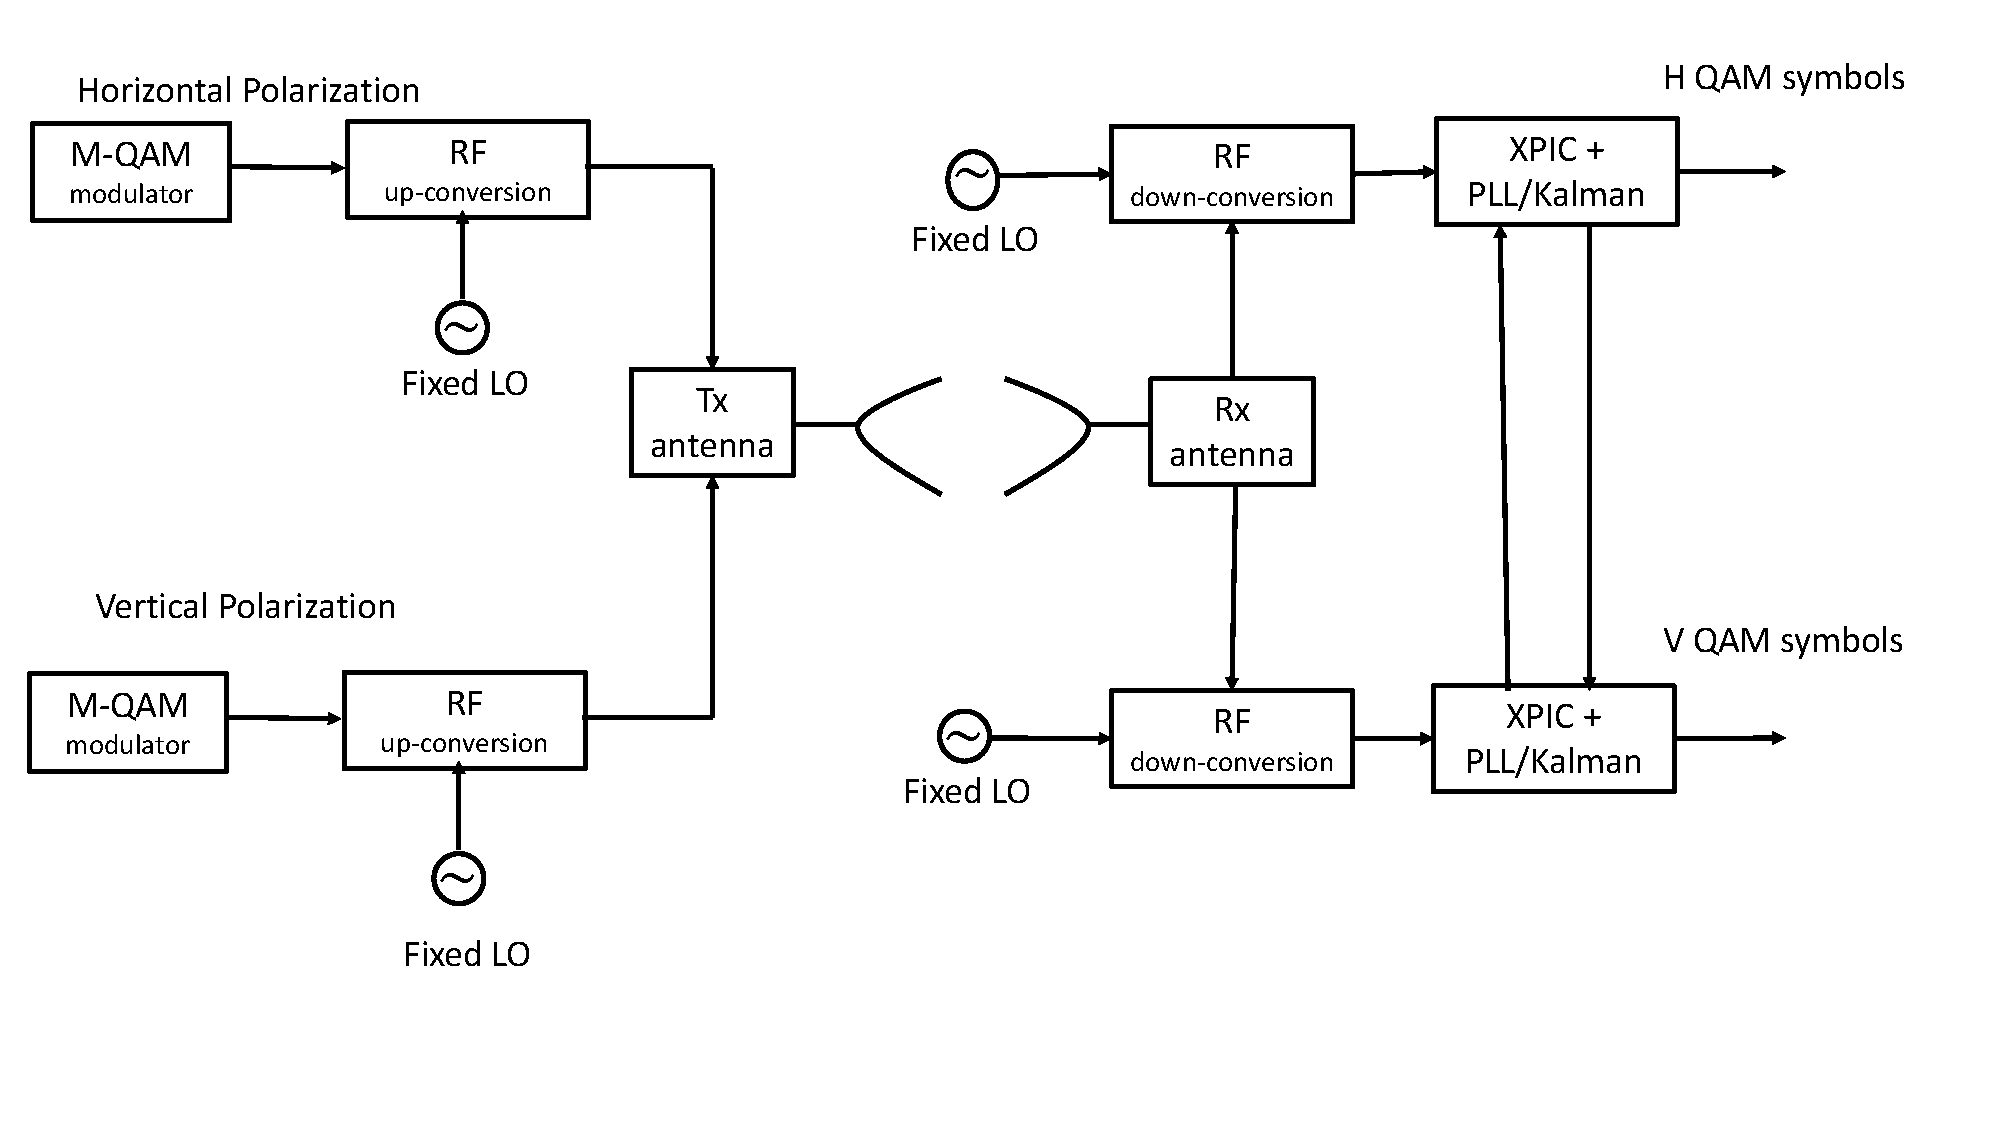
\includegraphics[width=1\textwidth]{figures/fig_red_kalman/Fig1.pdf}
	\caption{System Architecture}
	\label{Fig1}
\end{figure}


We consider a backhaul link with two distinct receiver paths and unsynchronized local oscillators (LO), as in \cite{Rossi}, \cite{CommLett}. Fig. \ref{Fig1} depicts the considered XPIC architecture, highlighting the two distinct receiver paths, with unsynchronized local oscillators (LO) for a backhaul link \cite{Rossi}. Since our focus is a typical microwave backhaul application, we model the channel with only AWGN without multipath fading as in \cite{CommLett}.

Let us consider the signal $r_0(n)$, received at one polarization path:

\begin{equation}
r_0(n)=t_0(n)e^{j\theta(n)}+gt_1(n)e^{j\phi(n)}+w(n)
\label{eq_r0}
\end{equation}

where $t_0(n)$ is the $n^{th}$ complex QAM transmitted symbol of the main polarization component with phase $\theta(n)$, $g$ is the cross-polar attenuation factor, $t_1(n)$ is the $n^{th}$ complex QAM symbol transmitted on the interference path with phase $\phi(n)$, and $w(n)$ represents the additive white Gaussian noise (AWGN) at the receiver.

The \textcolor{black}{aim} of both the Kalman and PLL algorithms is to estimate the phases ${\theta}(n)$ and  ${\phi}(n)$, along with the corresponding frequencies ${\dot{\theta}}(n)$ and ${\dot{\phi}}(n)$, by using the input of the main polarization slicer:
\begin{equation}
u_0(n)=\left(r_0(n)-gt_1(n)e^{-j\hat{\phi}(n)}\right)e^{-j\hat{\theta}(n)}
\label{outsig}
\end{equation}
where $\hat{\phi}(n)$ and $\hat{\theta}(n)$ represent the estimated phases of the main and cross polar signals at the receiver.
The cross-polar attenuation factor $\mathit{g}$ is assumed to be known, since, in high-order M-QAM receivers for microwave backhaul links, a linear filter interference canceller/equalizer is able to converge in presence of both baseband phase and frequency errors, providing a good initial guess for the PLL or the Kalman algorithms. Usually, during the acquisition phase, the adaptive linear filter works in a blind mode, typically by a constant modulus algorithm (CMA), and switches to a minimum mean square error (MMSE) algorithm once the normal operating condition is reached. Once the equalizer switches to MMSE, all the others recovery algorithms, like the Kalman phase recovery one, start using the decisions at the output of the slicer. 
In the following Sec. \ref{Kalm2state}, we give a short outline of the phase recovery using the two-state Kalman models \cite{CommLett}, and then, in Sec. \ref{KalmReduced}, we describe the proposed solutions, which include (i) a one-state Kalman model, (ii) a further simplified one-state version that uses a lower amount of information to recover the phase, and (iii) a downsampling of the covariance matrix computations to speed up the Kalman algorithm. All the proposed schemes aims to reduce the complexity of a Kalman based solution in a smart way in order to not degrade the performance. An alternative error computation \textcolor{black}{that can decrease the computational load of} Kalman implementation is also included, as well as some interesting relations between the Kalman and PLL parameters, useful for cross PLL parameters optimization, which is still missing.

\section{XPIC Phase Recovery Based on Kalman Filtering}

Since our purpose is to estimate the phase and the frequency of the signals in an XPIC scheme, such variables are considered in the Kalman state vectors.
We also define the observation vectors and the error to be minimized through the Kalman approach in order to obtain the estimates of the signal frequency and phase discrete values.\\	
Specifically, we consider a two-state XPIC Kalman algorithm for the main path and another one for the cross polar interference, so that the two-state vectors of the main and cross polar signals are expressed \cite{CommLett}:


%\setcounter{equation}{23}
\begin{equation}
\mathbf{x}_0(n)=\left[\begin{array}{c}
\theta(n)\\
\dot{\theta}(n)\\
\end{array}\right]
\label{eq_xx}
\end{equation}

\begin{equation}
\mathbf{x}_1(n)=\left[\begin{array}{c}
\phi(n)\\
\dot{\phi}(n)\\
\end{array}\right]
\label{eq_xx2}
\end{equation}

The state evolution of the linearized Kalman filter results:

%\setcounter{equation}{23}
\begin{equation}
\mathbf{x}_0(n)=\left[\begin{array}{c}
\theta(n)\\
\dot{\theta}(n)\\
\end{array}\right]=\mathbf{F}\left[\begin{array}{c}
\theta(n-1)\\
\dot{\theta}(n-1)\\
\end{array}\right]
\label{eq_xh}
\end{equation}

and

%\setcounter{equation}{24}
\begin{equation}
\mathbf{x}_1(n)=\left[\begin{array}{c}
\phi(n)\\
\dot{\phi}(n)\\
\end{array}\right]=\mathbf{F}\left[\begin{array}{c}
\phi(n-1)\\
\dot{\phi}(n-1)\\
\end{array}\right]
\label{eq_xv}
\end{equation}

where the transition matrix $\mathbf{F}$ is defined as

\begin{equation}
\mathbf{F}=\left[\begin{matrix}
1 & 1  \\
0 & 1  \\
\end{matrix}\right]
\label{eq_F2}
\end{equation}
The transition matrix definition $\mathbf{F}$ takes into account the fact that the residual carrier frequency offset at the PLL/Kalman input is usually lower than the initial one at the modem input, since a first stage coarse frequency detector is able to make it smaller. Moreover, the frequency offset time variations are anyway slower compared to the phase noise random fluctuations. 

While the cross polar observation vectors for the main and cross polarization signal, $\mathbf{r}_0(n)$ and $\mathbf{r}_1(n)$ respectively, are defined as

\begin{equation}
\begin{array}{ll}	
\mathbf{r}_0(n)=\mathbf{h}_0(\mathbf{x}_0(n))+\mathbf{w}_0(n)\\
\\
\mathbf{r}_1(n)=\mathbf{h}_1(\mathbf{x}_1(n))+\mathbf{w}_1(n)\\
\label{eq_r1}
\end{array}
\end{equation}
where
	\begin{equation}
	\mathbf{r}_0(n)=\left[\begin{array}{c}
	Re(\tilde{r}_0(n))\\
	Im(\tilde{r}_0(n))\\
	\end{array}\right],\;
	\mathbf{r}_1(n)=\left[\begin{array}{c}
	Re(g t_1(n))\\
	Im(g t_1(n))\\
	\end{array}\right]
	\label{eq_r}
	\end{equation}
	and $\mathbf{h}_0(\mathbf{x}_0(n))\doteq \mathbf{h}_0(n)$ and $\mathbf{h}_1(\mathbf{x}_1(n))\doteq \mathbf{h}_1(n)$ are the observer vectors, defined as
\begin{equation}
\mathbf{h}_0(n)=\left[\begin{array}{c}
\phantom{i}Re(\hat{t}_0(n)e^{j\theta(n)})\phantom{i}\\
\phantom{i}Im(\hat{t}_0(n)e^{j\theta(n)})\phantom{i}\\
\end{array}\right],\;
\mathbf{h}_1(n)=\left[\begin{array}{c}
Re(g\hat{t}_1(n)e^{j\phi(n)})\\
Im(g\hat{t}_1(n)e^{j\phi(n)})\\
\end{array}\right]
\label{eq_r}
\end{equation}
$\hat{t}_0(n)=\hat{a}(n)+j\hat{b}(n)$ is the output of the symbol \textcolor{black}{slicer}, $\tilde{r}_0(n)=r_0(n)-g\hat{t}_1(n)e^{-j\phi(n)}$, and:
\begin{equation}
\label{eq8}
g\hat{t}_1(n)e^{j\phi(n)}=r_0(n)-\hat{t}_0(n)e^{j\theta(n)}=\hat{c}(n)+j\hat{d}(n)
\end{equation}
While $\mathbf{w}_0(n)$ and $\mathbf{w}_1(n)$ are the observation noise on the main and interference path, respectively.
The EKF algorithms minimize the two distinct correspondent error vectors $\mathbf{e}_0(n)$ and $\mathbf{e}_1(n)$ defined as
\begin{equation}
\begin{array}{ll}	
\mathbf{e}_0(n)=\mathbf{r}_0(n)- \mathbf{h}_0(n)\\
\\
\mathbf{e}_1(n)=\mathbf{r}_1(n)- \mathbf{h}_1(n)\\
\label{eq_r2}
\end{array}
\end{equation}

The complete derivation of the EKF iterative equations may be found in section III of \cite{CommLett}.

\section{Proposed Reduced Complexity Kalman Algorithms}
\label{KalmReduced}

\subsection{One-State Kalman Model}
In this section, a simplified one-state Kalman model is developed for an XPIC scheme where only the phase of the signal is considered as state parameter, while the frequency is processed as an external input, obtaining a substantial complexity reduction. The proposed one-state model is derived starting from the two-state Kalman model \cite{CommLett}, in a way similar to the single-polarization scheme in \cite{Wei-Tsen}.

The one-state model can be represented as
%\setcounter{equation}{33}
\begin{equation}
\begin{array}{c}
x_0(n)=\theta(n)+\dot{\theta}(n)+v_0(n)\\
\\
x_1(n)=\phi(n)+\dot{\phi}(n)+v_1(n)\\
\end{array}
\label{eq_x1s}
\end{equation}
\textcolor{black}{where $v_0(n),v_1(n)$ represent the state noise signals.}
In the following we use the outputs of the hard decision 
$\hat{t}_0(n)=\hat{a}(n)+j\hat{b}(n)$ and $g\hat{t}_1(n)=\hat{c}(n)+j\hat{d}(n)$ 
to estimate the frequency $\dot{\theta}(n)$ and $\dot{\phi}(n)$. Note that the symbol $\hat{c}(n)+j\hat{d}(n)$ is always obtained from the slicer decisions of the main polarization component signal as follows:
\begin{equation}
\hat{c}(n)+j\hat{d}(n)=r_0(n)-\hat{t}_0(n)e^{j\hat{\theta}(n)}
\label{eq_gt12}
\end{equation}
which implies that the main path does not requires any feedback from the cross polar component, so that the two links work independently in a reciprocal blind manner.

The frequencies are computed by means of two first order loops:
\begin{equation}
\begin{array}{c}
\hat{\dot{\theta}}(n)=\hat{\dot{\theta}}(n-1)+K_{\theta i}Im\left\lbrace \textcolor{black}{u_0(n)}(\hat{a}(n)+j\hat{b}(n))^*\right\rbrace \\
\\
\hat{\dot{\phi}}(n)=\hat{\dot{\phi}}(n-1)+K_{\phi i}Im\left\lbrace \textcolor{black}{u_1(n)}(\hat{c}(n)+j\hat{d}(n))^*\right\rbrace \\
\label{eq_freq1s}
\end{array}
\end{equation}
where 
\begin{equation}
u_0(n)=(r_0(n)-gt_1(n)e^{-j\hat{\phi}(n)})e^{-j\hat{\theta}(n)}=\tilde{r}_0(n)e^{-j\hat{\theta}(n)}
\end{equation}
represents the phase corrected estimation of the main polarization received symbol, and $u_1(n)=-gt_1(n)e^{-j\hat{\phi}(n)}$ is the phase corrected estimation of the cross polar interference signal, according to (\ref{outsig}). $K_{\theta i}$, $K_{\phi i}$ are the integral gains which control the convergence rate of the frequency estimation algorithm and correspond to the integral loop parameter of a second-order PLL. $Im\left\lbrace . \right\rbrace $ is the imaginary part of its argument, while the symbol $^*$ represents the complex conjugate.

Equation (\ref{eq_freq1s}) is equivalent to a first-order PLL, so it has a lower performance compared to the complete two-state Kalman model described in Sec. \ref{Kalm2state}. Anyway, the complexity reduction makes its implementation \textcolor{black}{simpler} than a two-state Kalman scheme and comparable with a more common second-order PLL solution. 

The state equations for the one-state Kalman filter approach are given as follows in (\ref{eq_ph1s}), (\ref{eq_ph21s}):
%\setcounter{equation}{36}
\begin{equation}
\begin{array}{c}
\hat{\theta}(n|n)=\hat{\theta}(n|n-1)+\mathbf{K}_{\theta}\left(\mathbf{r}_0(n)-\mathbf{h}_0(n)\right)\\
\\
\hat{\phi}(n|n)=\hat{\phi}(n|n-1)+\mathbf{K}_{\phi}\left(\mathbf{r}_1(n)-\mathbf{h}_1(n)\right)\\
\label{eq_ph1s}
\end{array}
\end{equation}
%\setcounter{equation}{36}
\begin{equation}
\begin{array}{c}
\hat{\theta}(n+1|n)=\hat{\theta}(n|n)+\hat{\dot{\theta}}(n)\\
\\
\hat{\phi}(n+1|n)=\hat{\phi}(n|n)+\hat{\dot{\phi}}(n)\\
\label{eq_ph21s}
\end{array}
\end{equation}
where $\mathbf{K}_{\theta}(n)$, $\mathbf{K}_{\phi}(n)$ are the Kalman gains, while the errors are defined according to \textcolor{black}{the }equations (\ref{eq_r2}).

The one-state EKF may be derived according to
\begin{equation}
\begin{array}{c}
\mathbf{H}_0(n)=\dfrac{\delta \mathbf{h}_0}{\delta x_0}\arrowvert_{x_0=\hat{\theta}(n|n-1)}=\\
\\
=\left[ \begin{matrix} -\hat{a}(n)\sin(\hat{\theta}(n|n-1))-\hat{b}(n)\cos(\hat{\theta}(n|n-1))\\-\hat{b}(n)\sin(\hat{\theta}(n|n-1))+\hat{a}(n)\cos(\hat{\theta}(n|n-1))\end{matrix}\right]
\end{array}
\label{eq_H0s}
\end{equation}
\begin{equation}
\begin{array}{c}
\mathbf{H}_1(n)=\dfrac{\delta \mathbf{h}_1}{\delta x_1}\arrowvert_{x_1=\hat{\phi}(n|n-1)}=\\
\\
=\left[ \begin{matrix} -\hat{c}(n)\sin(\hat{\phi}(n|n-1))-\hat{d}(n)\cos(\hat{\phi}(n|n-1))\\-\hat{d}(n)\sin(\hat{\phi}(n|n-1))+\hat{c}(n)\cos(\hat{\phi}(n|n-1))\end{matrix}\right]
\end{array}
\label{eq_H1s}
\end{equation}

\subsubsection{One-State Model with Reduced Observations}
Following the same approach in \cite{Wei-Tsen}, it is possible to further reduce the implementation complexity by only considering the in-phase or the in-quadrature component in the two-dimensional equations (\ref{eq_r2},\ref{eq_ph1s},\ref{eq_H0s},\ref{eq_H1s}). 

\subsection{Alternative Error Detection Computation}
\label{Kalm2err}
In the following we formulate a new way of computing the minimized error in (\ref{eq_ph1s}), as an alternative to the model proposed in \cite{CommLett}, which provides the following main advantages:
\begin{itemize}
	\item it saves a phase counter-rotation in (\ref{eq_ph1s}) as shown in (\ref{err01}), which is usually hardware expensive;
	\item the one-state Kalman error is the same residual phase error used to drive the frequency estimations in (\ref{eq_freq1s}) which can be computed once for both the algorithms at each symbol time, thus saving computational operations.
\end{itemize}

The Kalman errors in (\ref{eq_ph1s}) corresponds to
\begin{equation}
\begin{array}{c}
e_0(n)=\tilde{r}_0(n)-\hat{t}_0(n)e^{j\hat{\theta}(n)}\\
e_1(n)=gt_1(n)-g\hat{t}_1(n)e^{j\hat{\phi}(n)}
\end{array}
\label{err01}
\end{equation}

In the following, we consider only the new error computation $\epsilon_0(n)$ corresponding to the main polarization error $e_0(n)$, since the same procedure can be replicated for $e_1(n)$.

The new computed error $\epsilon_0(n)$ is equal to the difference between the phases of the input and output of the symbol slicer as expressed in (\ref{eq_eps2_b}).

\begin{equation}
	\epsilon_0(n)=t_0(n)e^{-j\hat{\theta}(n)}(e^{j\theta(n)}-e^{j\hat{\theta}(n)})
	\label{eq_eps2_b}
\end{equation}

If we only consider the phase noise  contribution at the output of the interference canceler, the input of the main polarization slicer $u_0(n)$ in (2) can be recomputed as follows

\begin{equation}
u_0(n)=\tilde{r}_0(n)e^{-j\hat{\theta}(n)}=t_0(n)e^{j(\theta(n)-\hat{\theta}(n))}
\label{eq_s0_b}
\end{equation}
%
%Then, we calculate the new error detection $\epsilon(n)$ as
%
%\begin{equation}
%\epsilon(n)=\tilde{r}_0(n)e^{-j\hat{\theta}(n)}-\hat{t}_0(n)
%\label{eq_eps_b}
%\end{equation}
%
%which, under the hypothesis $\hat{t}_0(n)=t_0(n)$ becomes

Defining $s_0(n)$ as in the following

\begin{equation}
\begin{array}{lll}
s_0(n)=\epsilon_0^*(n)u_0(n)=\\
\\
\phantom{xxii}=|t_0(n)|^2e^{-j\hat{\theta}(n)}(e^{-j\theta(n)}-e^{-j\hat{\theta}(n)})e^{j(\theta(n)-\hat{\theta}(n))}=\\
\\
\phantom{xxii}=|t_0(n)|^2\left(-2j\sin\left(\frac{\Delta\theta}{2}\right)\right)e^{\frac{\Delta\theta(n)}{2}} 
\end{array}
\label{eq_u_b}
\end{equation}

where $\Delta\theta(n)=\theta(n)-\hat{\theta}(n)$ represents the difference between the true phase and the estimated one, i.e. the phase error at the output of the slicer. $\Delta\theta(n)$ may be computed, as usual in digital PLL, as in (\ref{eq_ph1s}).

Being $Im\left[u_0(n)\right]=-2\cos(\frac{\Delta\theta(n)}{2})\sin(\frac{\Delta\theta(n)}{2})=-2\sin\left(\frac{\Delta\theta}{2}\right)$, $\mathbf{H}_0(n)$ may be computed as $\dfrac{\delta(u_0(n))}{\delta\theta}$ so that
\begin{equation}
\begin{array}{c}
\mathbf{H}_0(n)=\left[\begin{matrix}
-\hat{a}(n)\sin(\Delta\theta(n))-\hat{b}(n)\cos(\Delta\theta(n))\\
-\hat{b}(n)\sin(\Delta\theta(n))+\hat{a}(n)\cos(\Delta\theta(n)) \\
\end{matrix}\right]
\end{array}
\label{eq_ssH0new_b}
\end{equation}

Similarly, it is possible to compute $\mathbf{H}_1(n)$ as follows
\begin{equation}
\begin{array}{c}
\mathbf{H}_1(n)=\left[\begin{matrix}
-\hat{c}(n)\sin(\Delta\phi(n))-\hat{d}(n)\cos(\Delta\phi(n))  \\
-\hat{d}(n)\sin(\Delta\phi(n))+\hat{c}(n)\cos(\Delta\phi(n))  \\
\end{matrix}\right]
\end{array}
\label{eq_ssH1new_b}
\end{equation}

% and to calculate the state evolution equations for the cross polar signal.
As final remark, such alternative error detection computation has the benefit to avoid the \textcolor{black}{hardware cost of a} phase counter-rotation in (\ref{err01}).


Fig. \ref{Hnew_fig} summarizes the steps described above.


\begin{figure}
	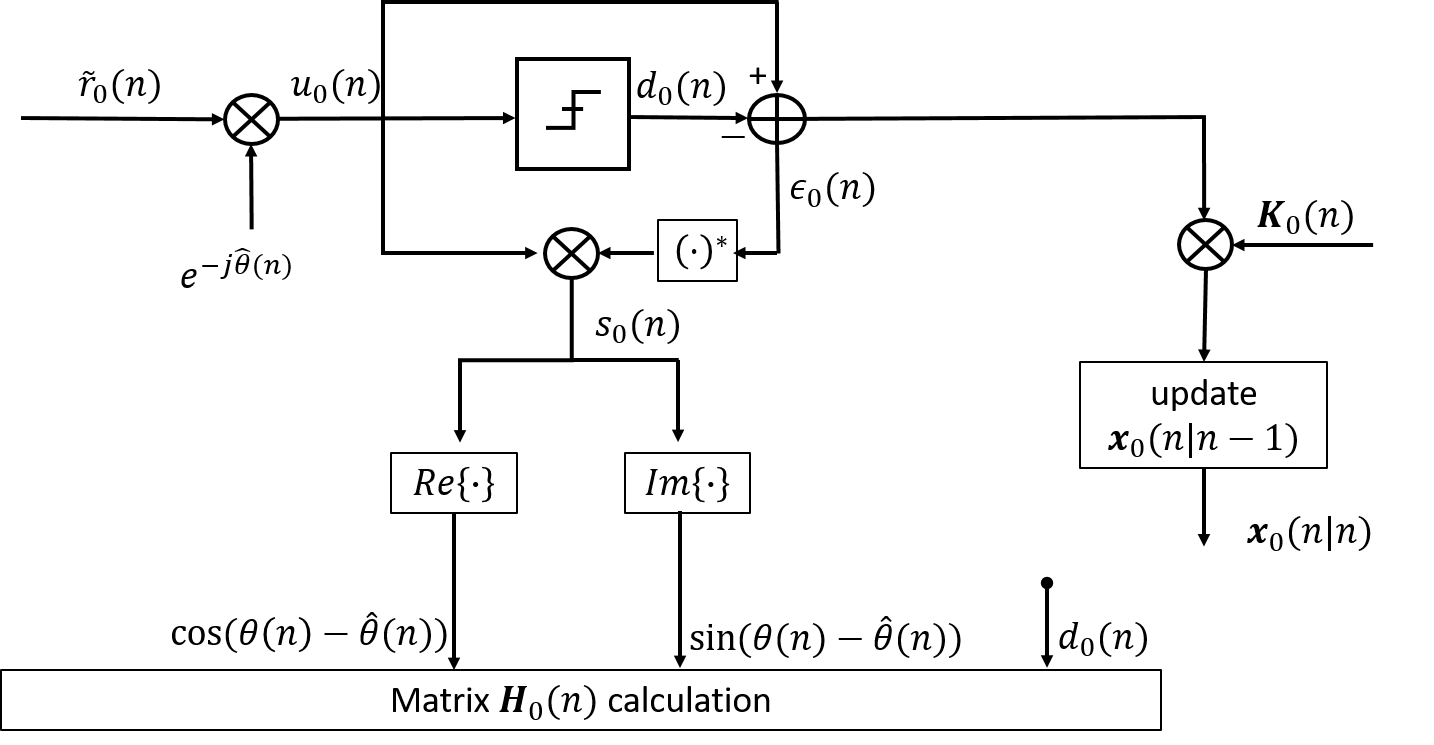
\includegraphics[width=0.9\textwidth]{figures/fig_red_kalman/Hnew.png}
	\caption{Kalman model with the alternative error detection}
	\label{Hnew_fig}      
\end{figure}

\subsection{EKF Algorithm with covariance matrix loop downsampling}
\label{SecDSF}
Since the implementation of a Kalman filter for phase and frequency recovery is computationally expensive from an hardware point of view, we also consider a simplified approach where the covariance matrix computation loop is downsampled in time in order to speed up the algorithm and reduce its complexity. 

Simulation results have shown that it is possible to keep almost the same performance by increasing the downsampling factor up to 64, for all the presented results.

\subsection{Relation between the Extended Kalman approach and a digital PLL}
\label{KalmRelationPLL}

In this section we analyze the relation between the Extended Kalman and PLL parameters, which is of more importance for the estimation of the PLL interference phase, since it is not possible to use a closed form solution in order to estimate them in a cross scheme. Indeed, it is possible to derive closed form solutions for PLL parameters optimization only for single-carrier architectures.



While \cite{Patapoutian} expresses the relation between Kalman filter and proportional-integral PLL, following a similar structures, we derive the relation (\ref{eq_pllK}) between the Extended Kalman version and PLL.
Since we refer to an XPIC scheme, the equation considers both the main and cross polar component:

\begin{equation}
\begin{array}{c}
\left[ \begin{array}{c} \alpha_{0p}\\\alpha_{0i}\end{array}\right] 	 =E[\mathbf{K}_0\mathbf{H}_0]\\
\\
\left[ \begin{array}{c} \alpha_{1p}\\\alpha_{1i}\end{array}\right] 	 =E[\mathbf{K}_1 \mathbf{H}_1]
\end{array}	
\label{eq_pllK}
\end{equation}
where $\alpha_{0p}$ and $\alpha_{0i}$ are the proportional-integral PLL gains for the main component,  $\alpha_{1p}$ and $\alpha_{1i}$ the cross polar component gains.
 
$\mathbf{K}_0$ and $\mathbf{K}_1$ are the Kalman gain matrices of the main and cross polar component, respectively. Finally,  $\mathbf{H}_0$ and $\mathbf{H}_1$, calculated as in (\ref{eq_ssH0new_b})-(\ref{eq_ssH1new_b}), are the contributions that account for the linearization of the EKF.

The calculation of the expected value converges in a few tens of symbols.

The reliability of the proposed method has been validated on the main path by using the closed form PLL equations, and by simulations for the cross-polar phase recovery path.

\section{Simulation Results}
\label{Results}

\subsection{Simulation Environment}
\label{SE}
For comparison purpose, we have considered the same simulation environment  of \cite{CommLett}:
\begin{itemize}
	\item a $1024$-QAM modulation for both the main signal and the cross polar interferer;
	\item symbol rate equal to 25 MHz;
	\item phase noise parameters for both polarizations: -67 dBc/Hz at 10 KHz, -96 dBc/Hz at 100 KHz;
	\item the loop gains of the two PLLs, and the integral ones of the proposed scheme are set by using equations (\ref{eq_pllK}): $K_{\theta i}=\alpha_{0i}$, $K_{\phi i}=\alpha_{1i}$;
	\item periodical transmission of known constellation corner symbol pilots every 55 transmitted symbols.
\end{itemize}
As in \cite{CommLett}, the phase noise parameters and the $E_b/N_0$ are used to compute the covariances of the noise signals ${v}_0(n)$, ${v}_1(n)$, $\mathbf{w}_0(n)$ and $\mathbf{w}_1(n)$.

\subsection{BER Performance Evaluation}
\label{PE}
\begin{figure}
	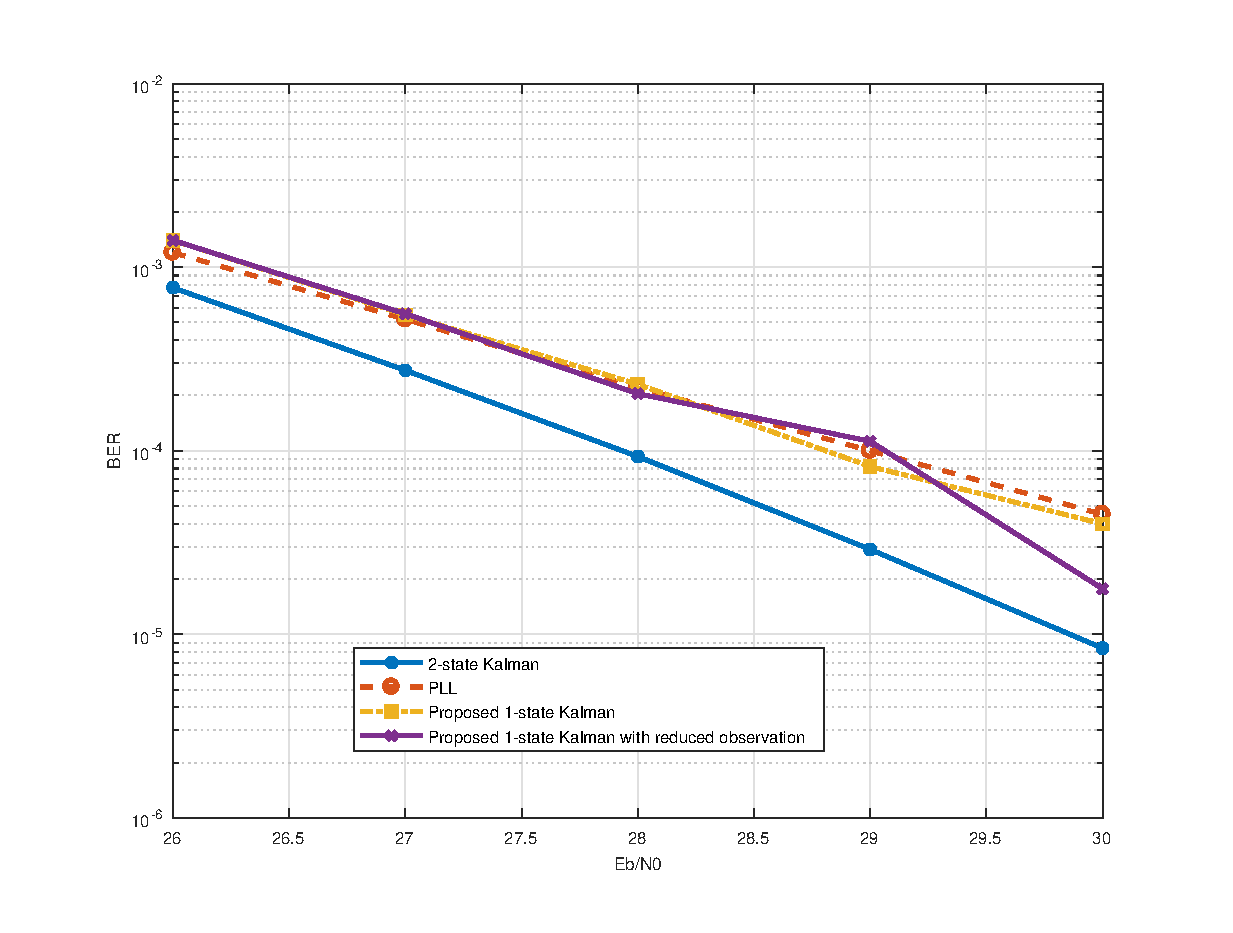
\includegraphics[width=1\textwidth]{figures/fig_red_kalman/Fig3.eps}
	\caption{BER evaluation: 1024 QAM and XPD=15 dB.
		The parameters of all the algorithms are optimized for $XPD=15$ dB, $E_b/N_0=26$ dB.}
	\label{fig3}      
\end{figure}
The bit error rate (BER) of the proposed reduced complexity Kalman based solutions are compared with both the two-state Kalman model and the second-order PLL one: the parameters of the second-order PLL and the
Kalman algorithms are optimized for $Eb/N0 = 26$ dB and $XPD=15$ dB.
\begin{figure}
	\includegraphics[width=0.8\textwidth]{figures/fig_red_kalman/Fig4.eps}
	\caption{BER evaluation: 1024 QAM and $XPD=25$ dB, while the parameters of all the algorithms are optimized for $XPD=15$ dB, $E_b/N_0=26$ dB.}
	\label{fig4}      
\end{figure}

Fig. \ref{fig3},\ref{fig4} show that, despite their lower complexity, the developed one-state Kalman models show similar or even better performance than the typical PLL architecture. However, as expected, the two-state Kalman solution outperforms the one-state algorithms, at the cost of higher complexity. Going in more details, Fig. \ref{fig3} illustrates the BER when the gains of both Kalman and PLL solutions are optimized for known value of the interference parameter $XPD=15$ dB, i. e. it is assumed no mismatch between such parameter estimation and its real value. Under this condition, the proposed one-state Kalman solutions perform slightly better than the common second-order PLL. Moreover, as shown in Fig. \ref{fig4}, the proposed algorithms are less sensitive to carrier-to-interference variations. Indeed, when the real $XPD$ value is different from the one used to optimize the algorithm parameters as in Fig. \ref{fig4}, both the proposed one-state Kalman versions perform much better than the commonly used second-order PLL scheme.

\subsection{Computational Complexity Evaluation}
\label{PEC}

Table \ref{table:1} illustrates the different matrix dimensions of the Kalman based solutions to show a computational complexity comparison.

\begin{table}[h!]
	\caption{ Computational complexity comparison in terms of matrix dimensions in Kalman based solutions.}
	\centering
	%	\setlength{\arrayrulewidth}{.15em}
	%\begin{tabular}{ p{1.5cm} p{1.5cm} p{1.5cm} p{2.5cm}   }
	\begin{tabular}{cccc}
		\hline
		\centering
		Matrix & 2-state Kalman  & 1-state Kalman & 1-state Kalman with\\
		& & & reduced observation\\
		\hline
		$\mathbf{H}$   & 2x2  &1x2&  1x1\\
		$\mathbf{K}$   &   2x2  & 2x1 &  1x1\\
		$\mathbf{Q}_{v}$ &2x2 &1x1&  1x1\\
		$\mathbf{Q}_{w}$ &2x2 &1x1&  1x1\\
		$\mathbf{R}$    &2x2 &2x2&  1x1\\
		$\mathbf{F}$ &   2x2  & 1x1&1x1\\
		\hline	
	\end{tabular}
	
	\hfill \break
	\label{table:1} 	
\end{table}


Furthermore, Fig. \ref{fig5}-\ref{fig8} compare the complexity of Kalman based solutions showing the computational times needed to calculate the Kalman gains $\mathbf{K}$, the covariance matrix  $\mathbf{R}$, and the innovation covariance inverse $\mathbf{S}^{-1}$, respectively. Indeed, the computation of such variables represents the most expensive operation for EKF algorithms, due to the Jacobian matrices of equations (\ref{eq_ssH0new_b}-\ref{eq_ssH1new_b}).
Fig. \ref{fig5}-\ref{fig8} confirm that both the proposed one-state Kalman model and its one-state version with reduced observation require less computation time compared to the two-state scheme. In particular, the one-state scheme with reduced observation demands the minimum computation time since all the Kalman parameters become scalars. As shown in Fig. \ref{fig3}-\ref{fig4} such advantage of the proposed one-state model solutions is achieved at the cost of lower performance compared to the two-state Kalman approach. However, their performance are comparable and even better of the commonly used second-order PLL scheme.
\begin{figure}
	\includegraphics[width=0.85\textwidth]{figures/fig_red_kalman/Fig5.eps}
	\caption{Simulation time comparison for the Kalman gains $\mathbf{K}$ calculation: 2-state Kalman, 1-state Kalman and 1-state Kalman with reduced observation.}
	\label{fig5}      
\end{figure}
\begin{figure}
	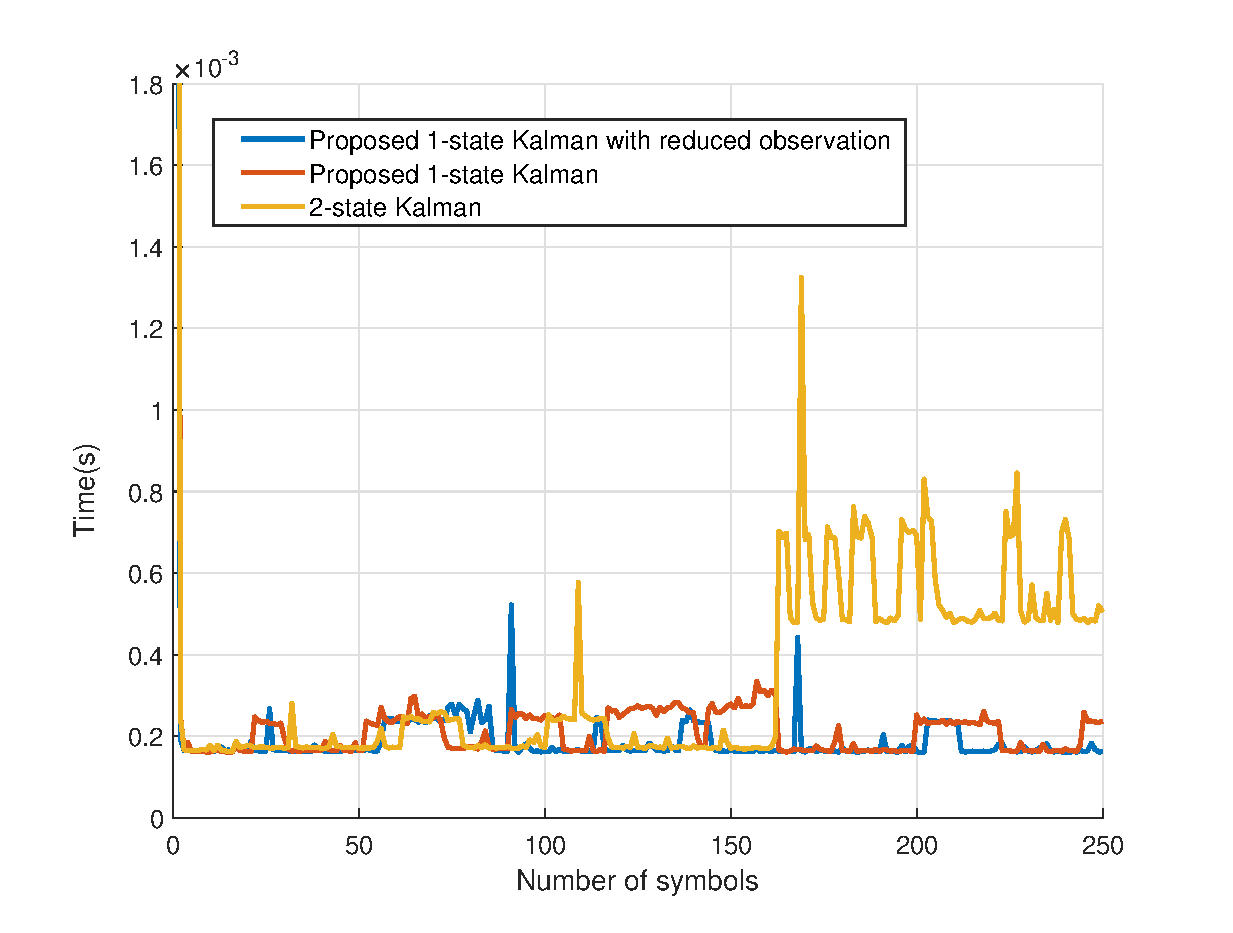
\includegraphics[width=0.85\textwidth]{figures/fig_red_kalman/Fig6bis.eps}
	\caption{Simulation time comparison for the innovation covariance matrix inverse $\boldsymbol{S}^{-1}$ calculation: 2-state Kalman, 1-state Kalman and 1-state Kalman with reduced observation.}
	\label{fig6}      
\end{figure}

\begin{figure}
	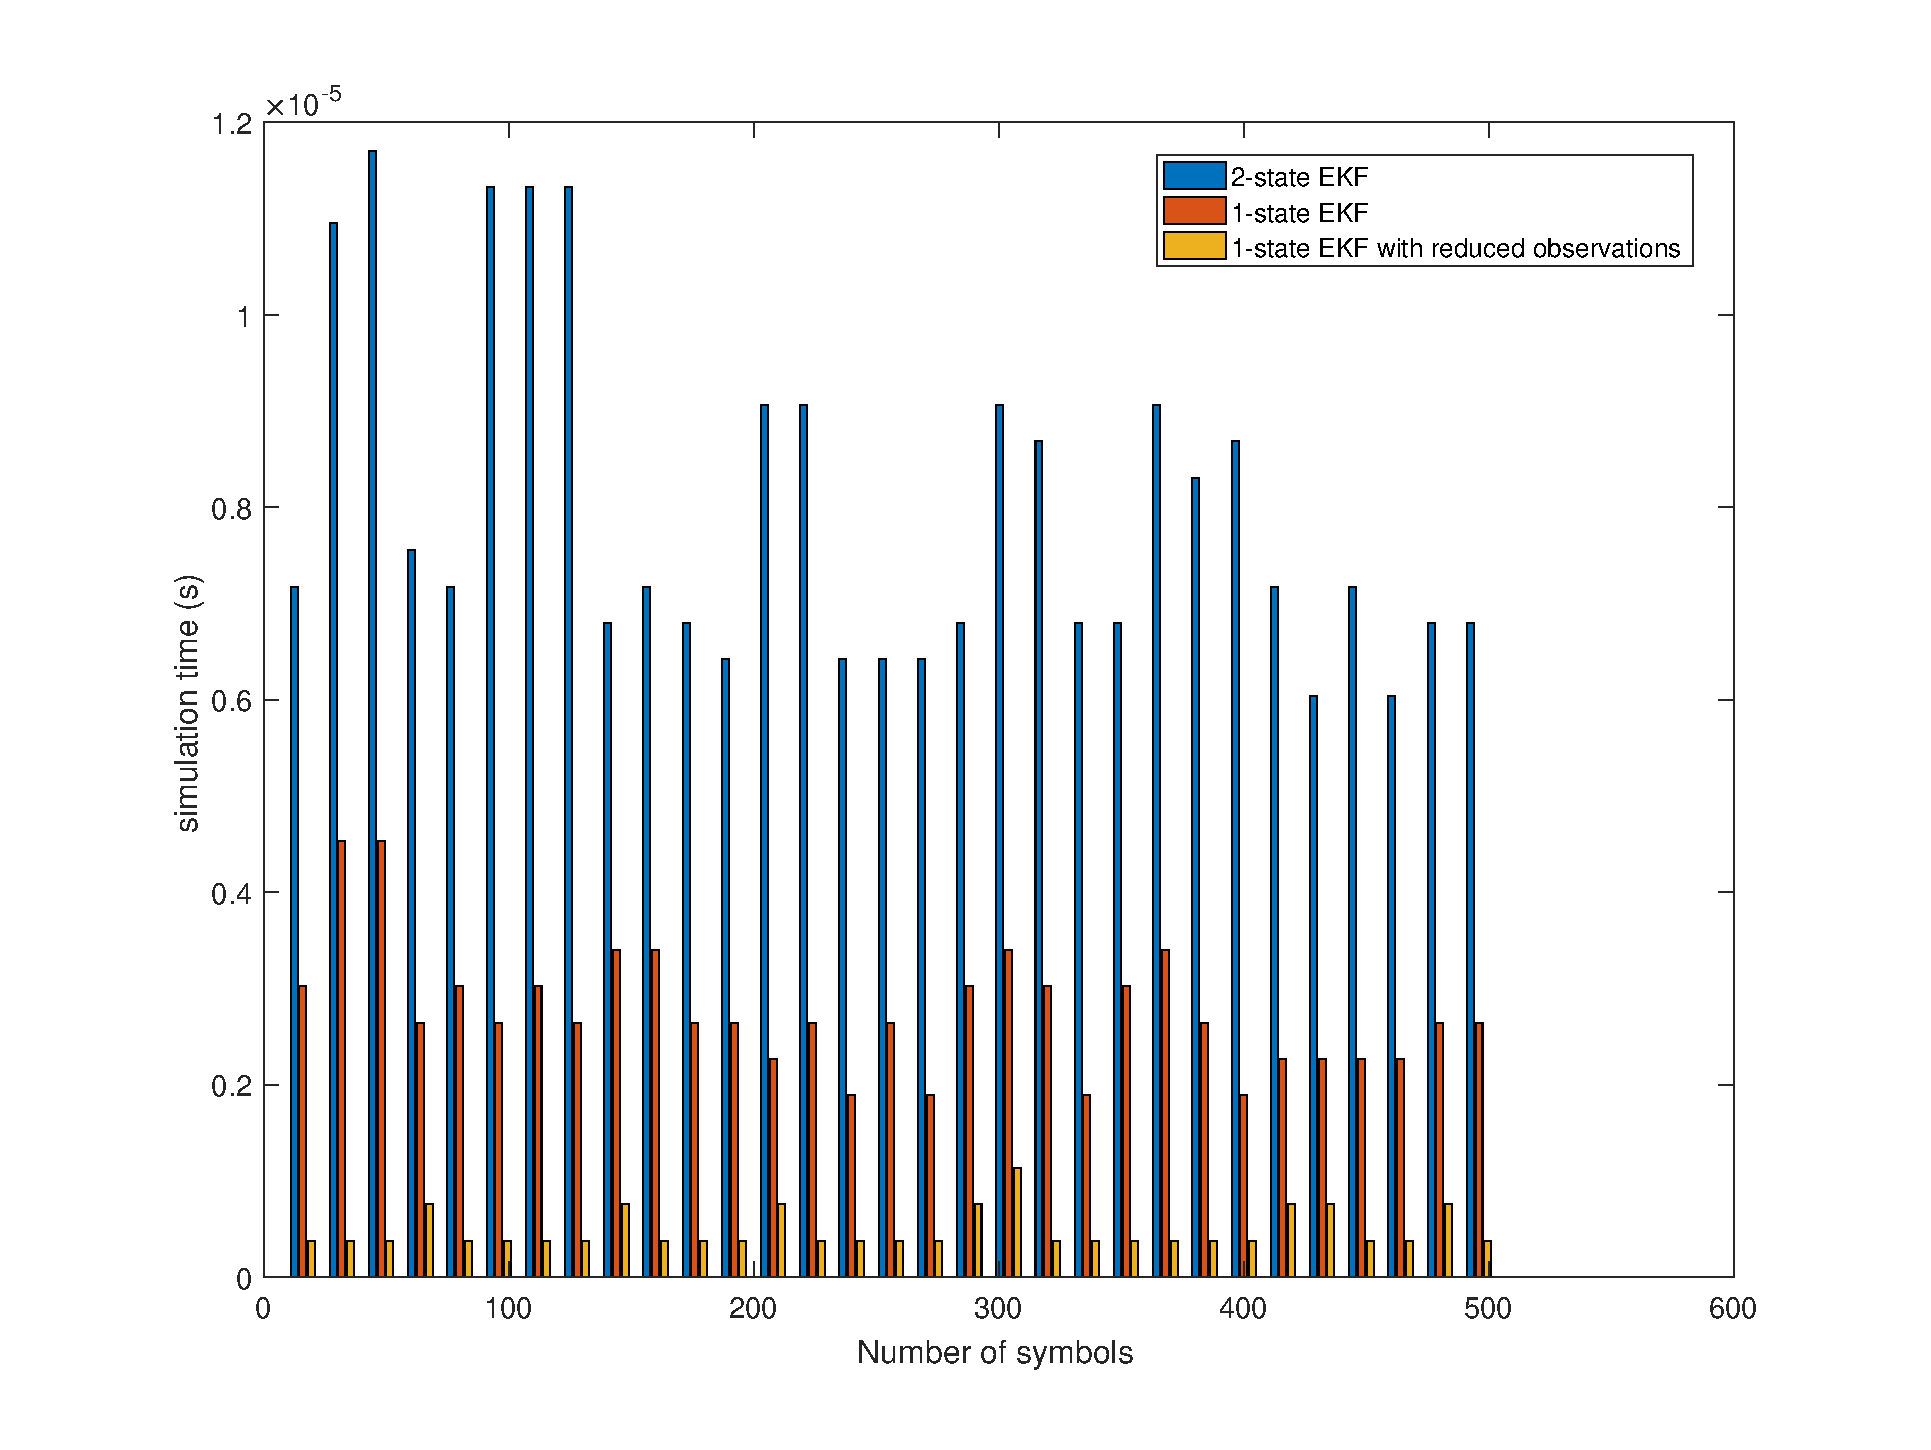
\includegraphics[width=0.85\textwidth]{figures/fig_red_kalman/Fig8.eps}
	\caption{Simulation time comparison for the Error Covariance matrix $\mathbf{R}$ calculation (Measurement update equation): 2-state Kalman, 1-state Kalman and 1-state Kalman with reduced observation.} 
	\label{fig8}      
\end{figure}

\subsection{Performance Evaluation of the downsampling covariance matrix}
\label{PEDSF}
As reported in the previous Sec. \ref{SecDSF}, hardware complexity can be further reduced by not updating the covariance matrix $\mathbf{R}(n)$ at each step without degrading the performance as shown in the following.
Fig. \ref{fig9_a} illustrates the BER performance of the proposed one-state Kalman for different \textcolor{black}{downsampling factors (DSFs)}, showing that the algorithm works well also for high DSF values. 

\begin{figure}
	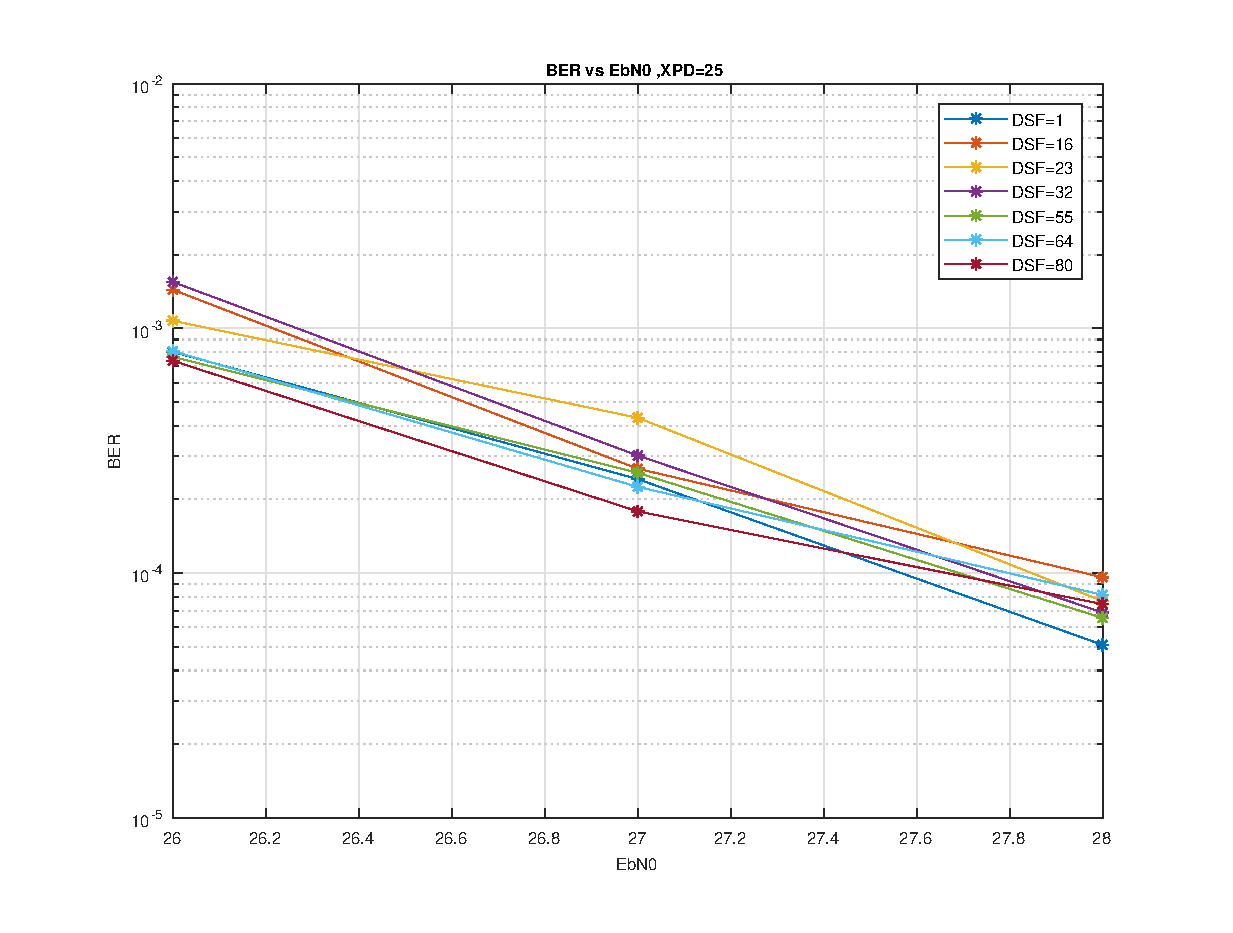
\includegraphics[width=0.85\textwidth]{figures/fig_red_kalman/Fig9_a.eps}
	\caption{BER for 1-state Kalman with different DSF, pilot interval=$56$, $XPD=25$ dB.}
	\label{fig9_a}      
\end{figure}

Being the concept of downsampling applicable also to other algorithms, in Fig. \ref{fig9}-\ref{fig15}, a comprehensive analysis has been performed for the two-state Kalman model with different DSFs, pilot intervals. Fig. \ref{fig9} shows the BER performance for different DSFs, with a pilot separation distance equal to $56$, while the pilot separation is $64$ in Fig. \ref{fig10}.

\begin{figure}
	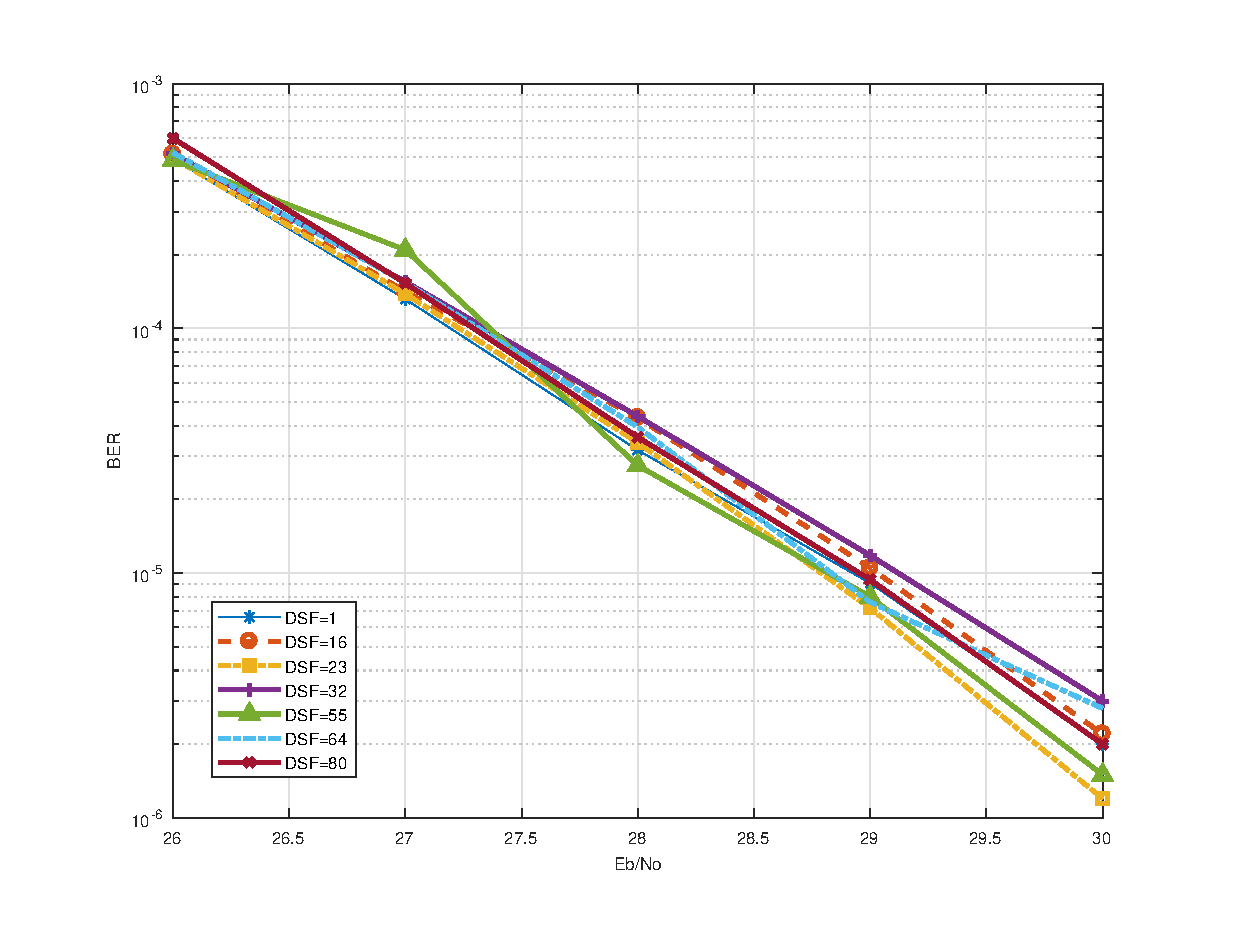
\includegraphics[width=0.85\textwidth]{figures/fig_red_kalman/Fig9.eps}
	\caption{BER for 2-state Kalman with different DSF, Pilot interval=$56$, $XPD=25$ dB.}
	\label{fig9}      
\end{figure}	
\begin{figure}
	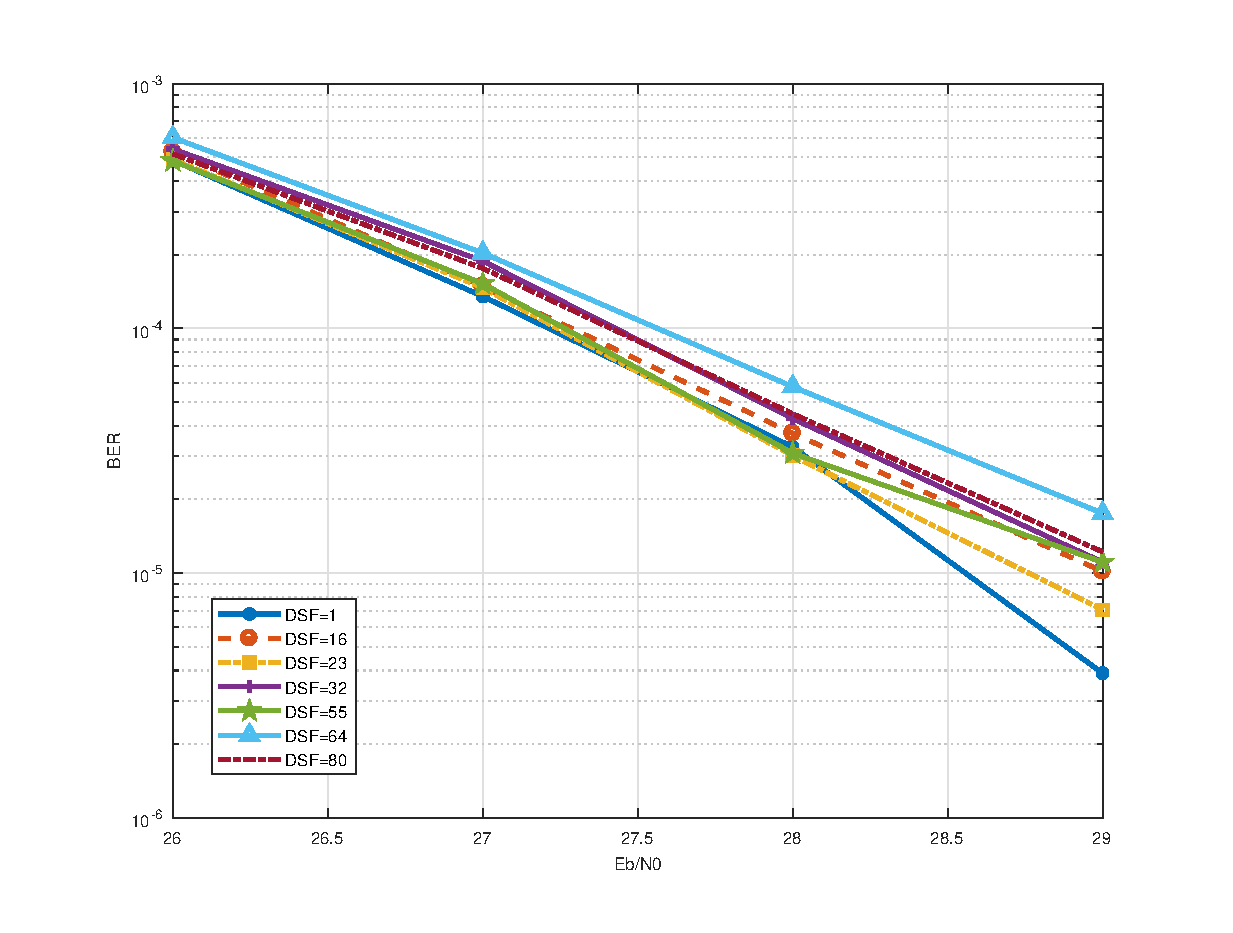
\includegraphics[width=0.85\textwidth]{figures/fig_red_kalman/Fig10.eps}
	\caption{BER for 2-state Kalman with different DSF, Pilot interval=$64$, $XPD=25$ dB.}
	\label{fig10}      
\end{figure}

As expected, comparing Fig. \ref{fig9} and \ref{fig10}, the best results are obtained with a lower pilot separation distance equal to $56$ symbols as in Fig. \ref{fig9}. Anyway, in both figures the scheme still show good performance till the highest value $DSF=80$.

Fig. \ref{fig11} illustrates BER performance for higher $DSF$ values showing that a $DSF$ greater than $80$ produces some unstable behavior in the system, so that, under this channel condition, $DSF=80$ could be considered as a performance upper limit.

\begin{figure}
	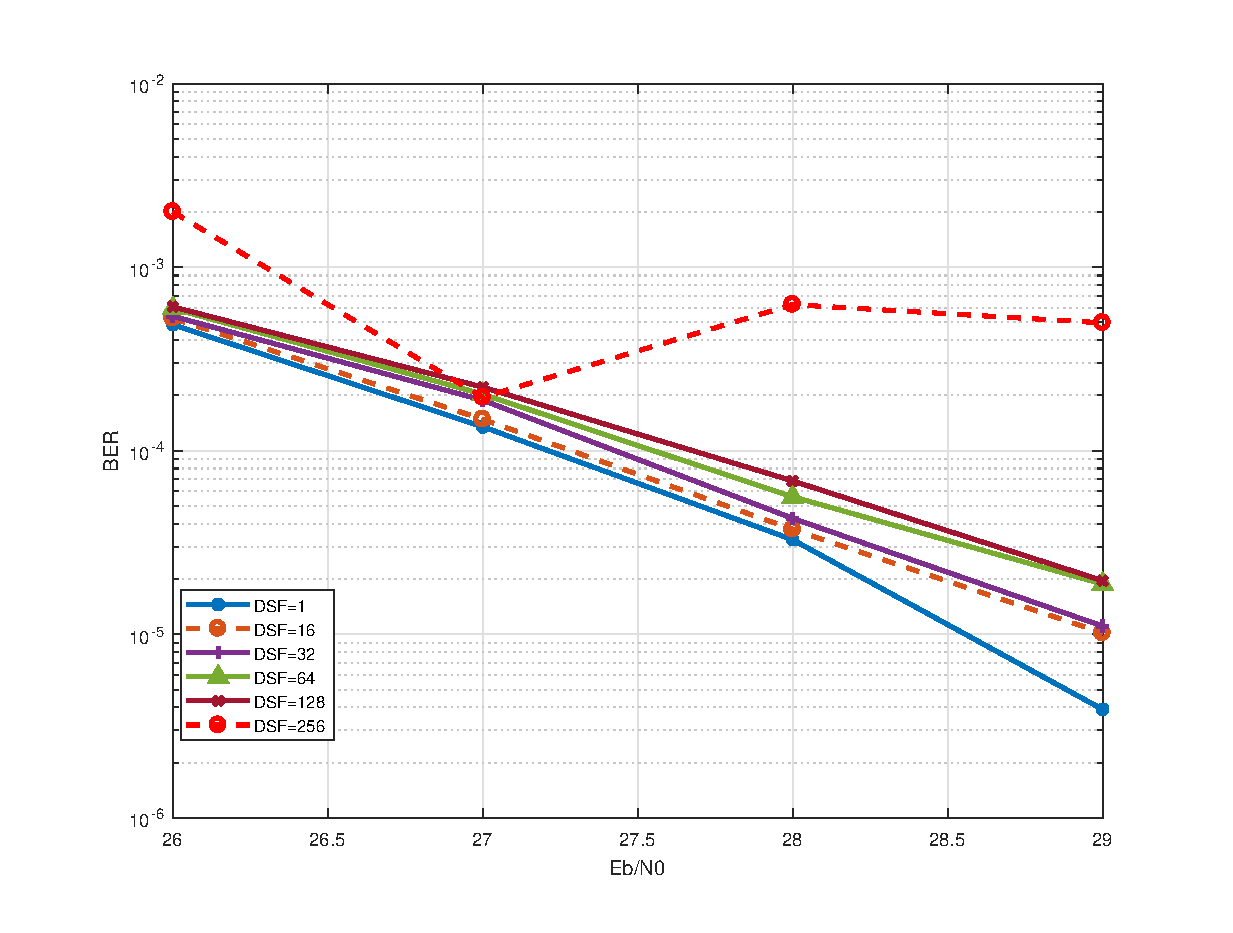
\includegraphics[width=0.85\textwidth]{figures/fig_red_kalman/fig11.eps}
	\caption{BER for 2-state Kalman with different DSF, pilot interval$=56$, $XPD=25$ dB.}
	\label{fig11}      
\end{figure}

Finally in the following Fig. \ref{fig12}-\ref{fig15}, we show BER performance when changing the modulation order. Instead of using a $1024$-QAM scheme as in all the previous results, Fig. \ref{fig12}-\ref{fig15} consider $64$-QAM and $256$-QAM for both $XPD=15$ dB and $XPD=25$ dB, showing more stable performance compared to the $1024$ order when increasing the downsampling factor. 

\begin{figure}
	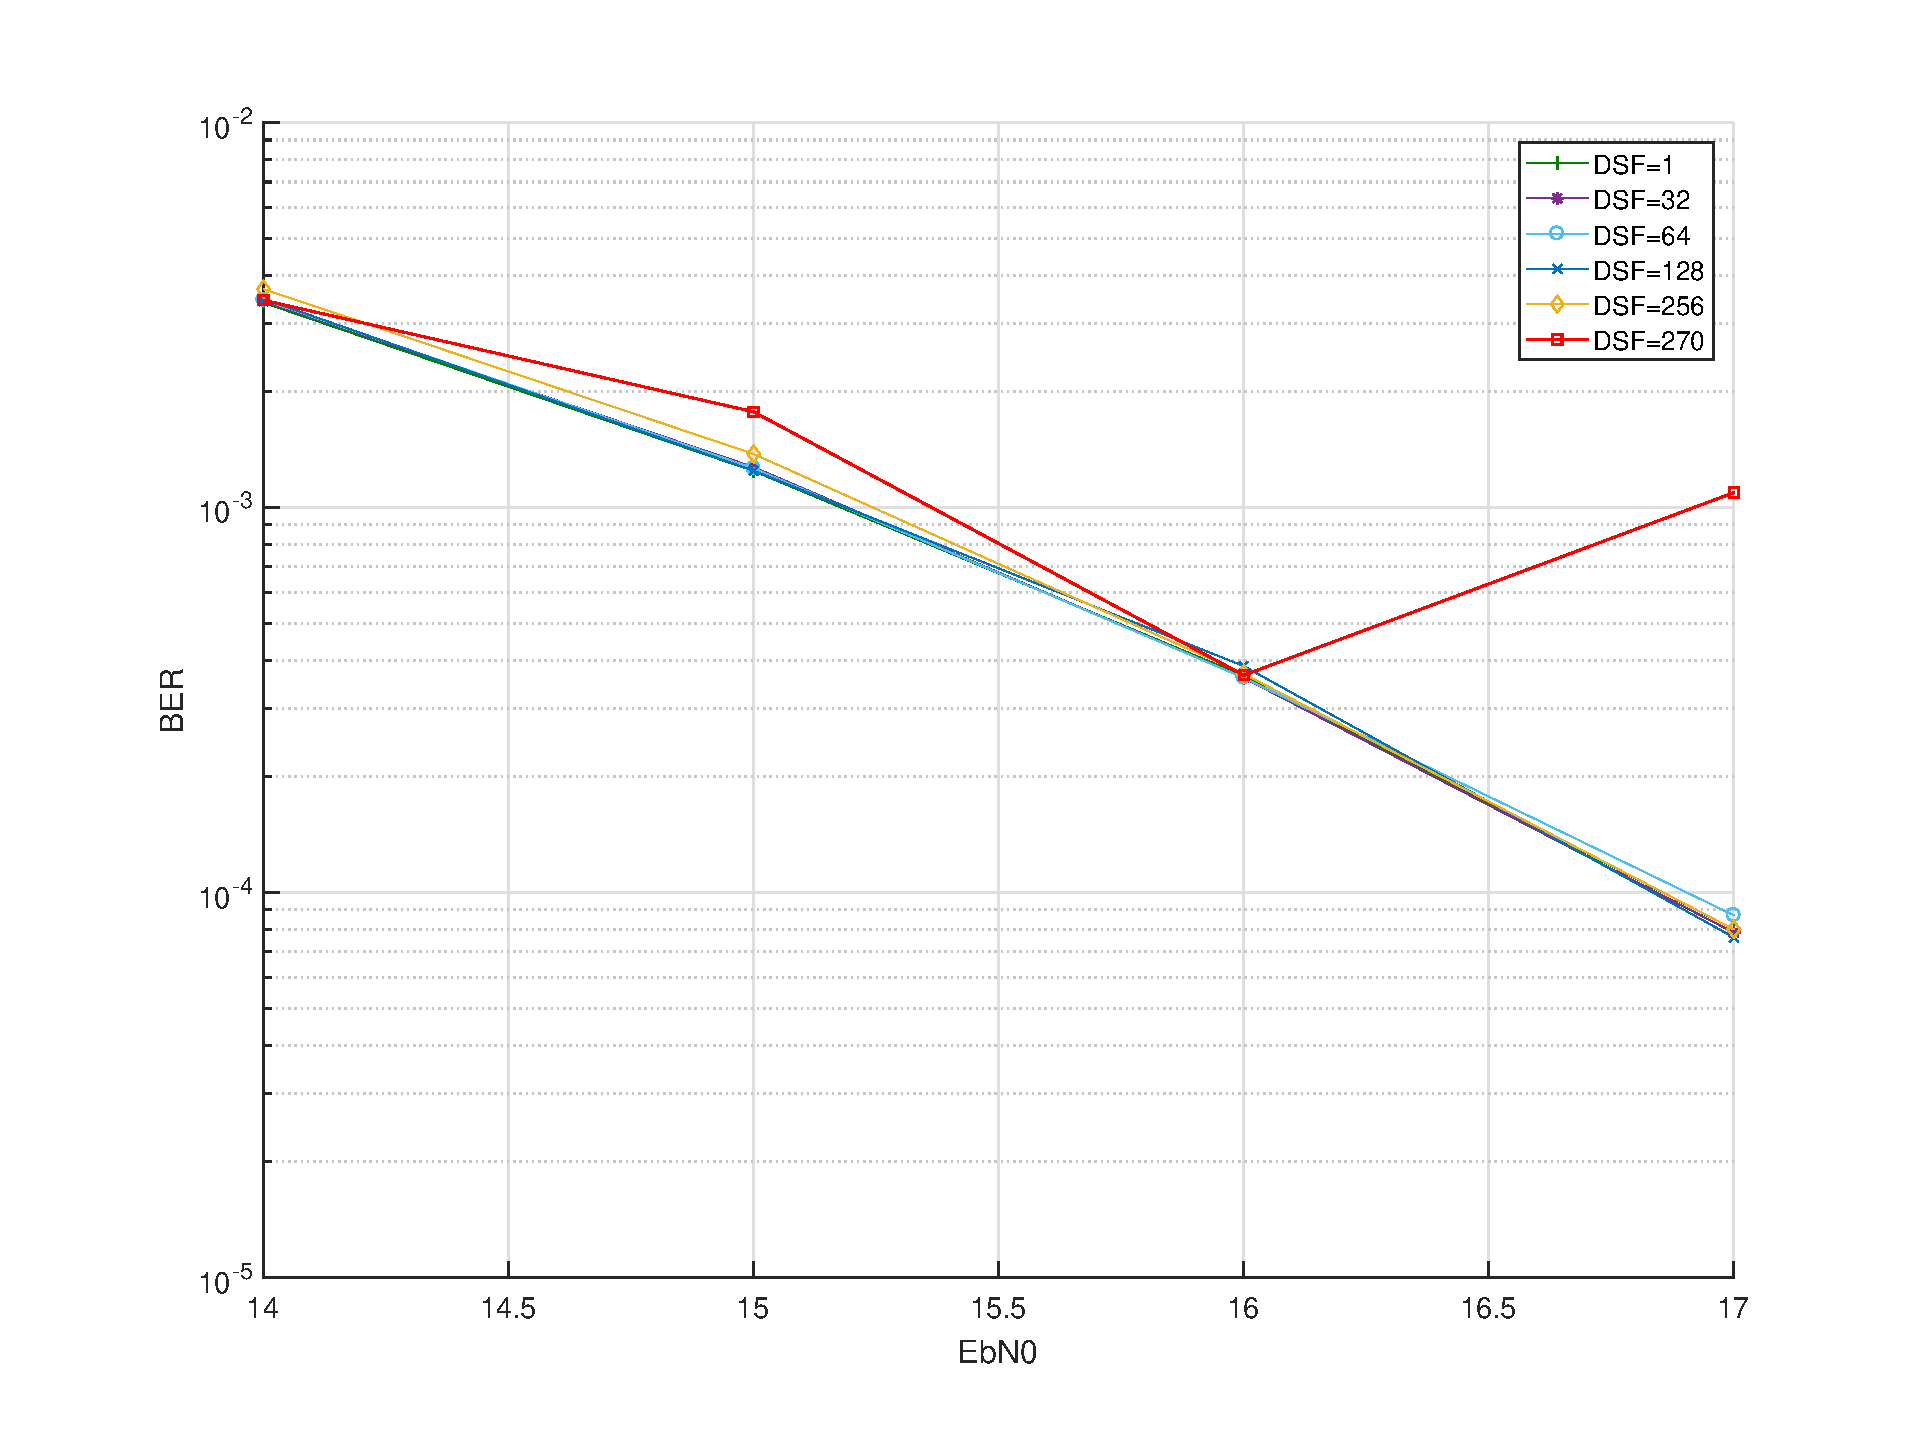
\includegraphics[width=0.85\textwidth]{figures/fig_red_kalman/xpic_xpd_15_qam_64_bis.eps}
	\caption{BER for 2-state Kalman with different DSF. $64$-QAM, $XPD=15$ dB, pilot interval=56.}
	\label{fig12}      
\end{figure}

\begin{figure}
	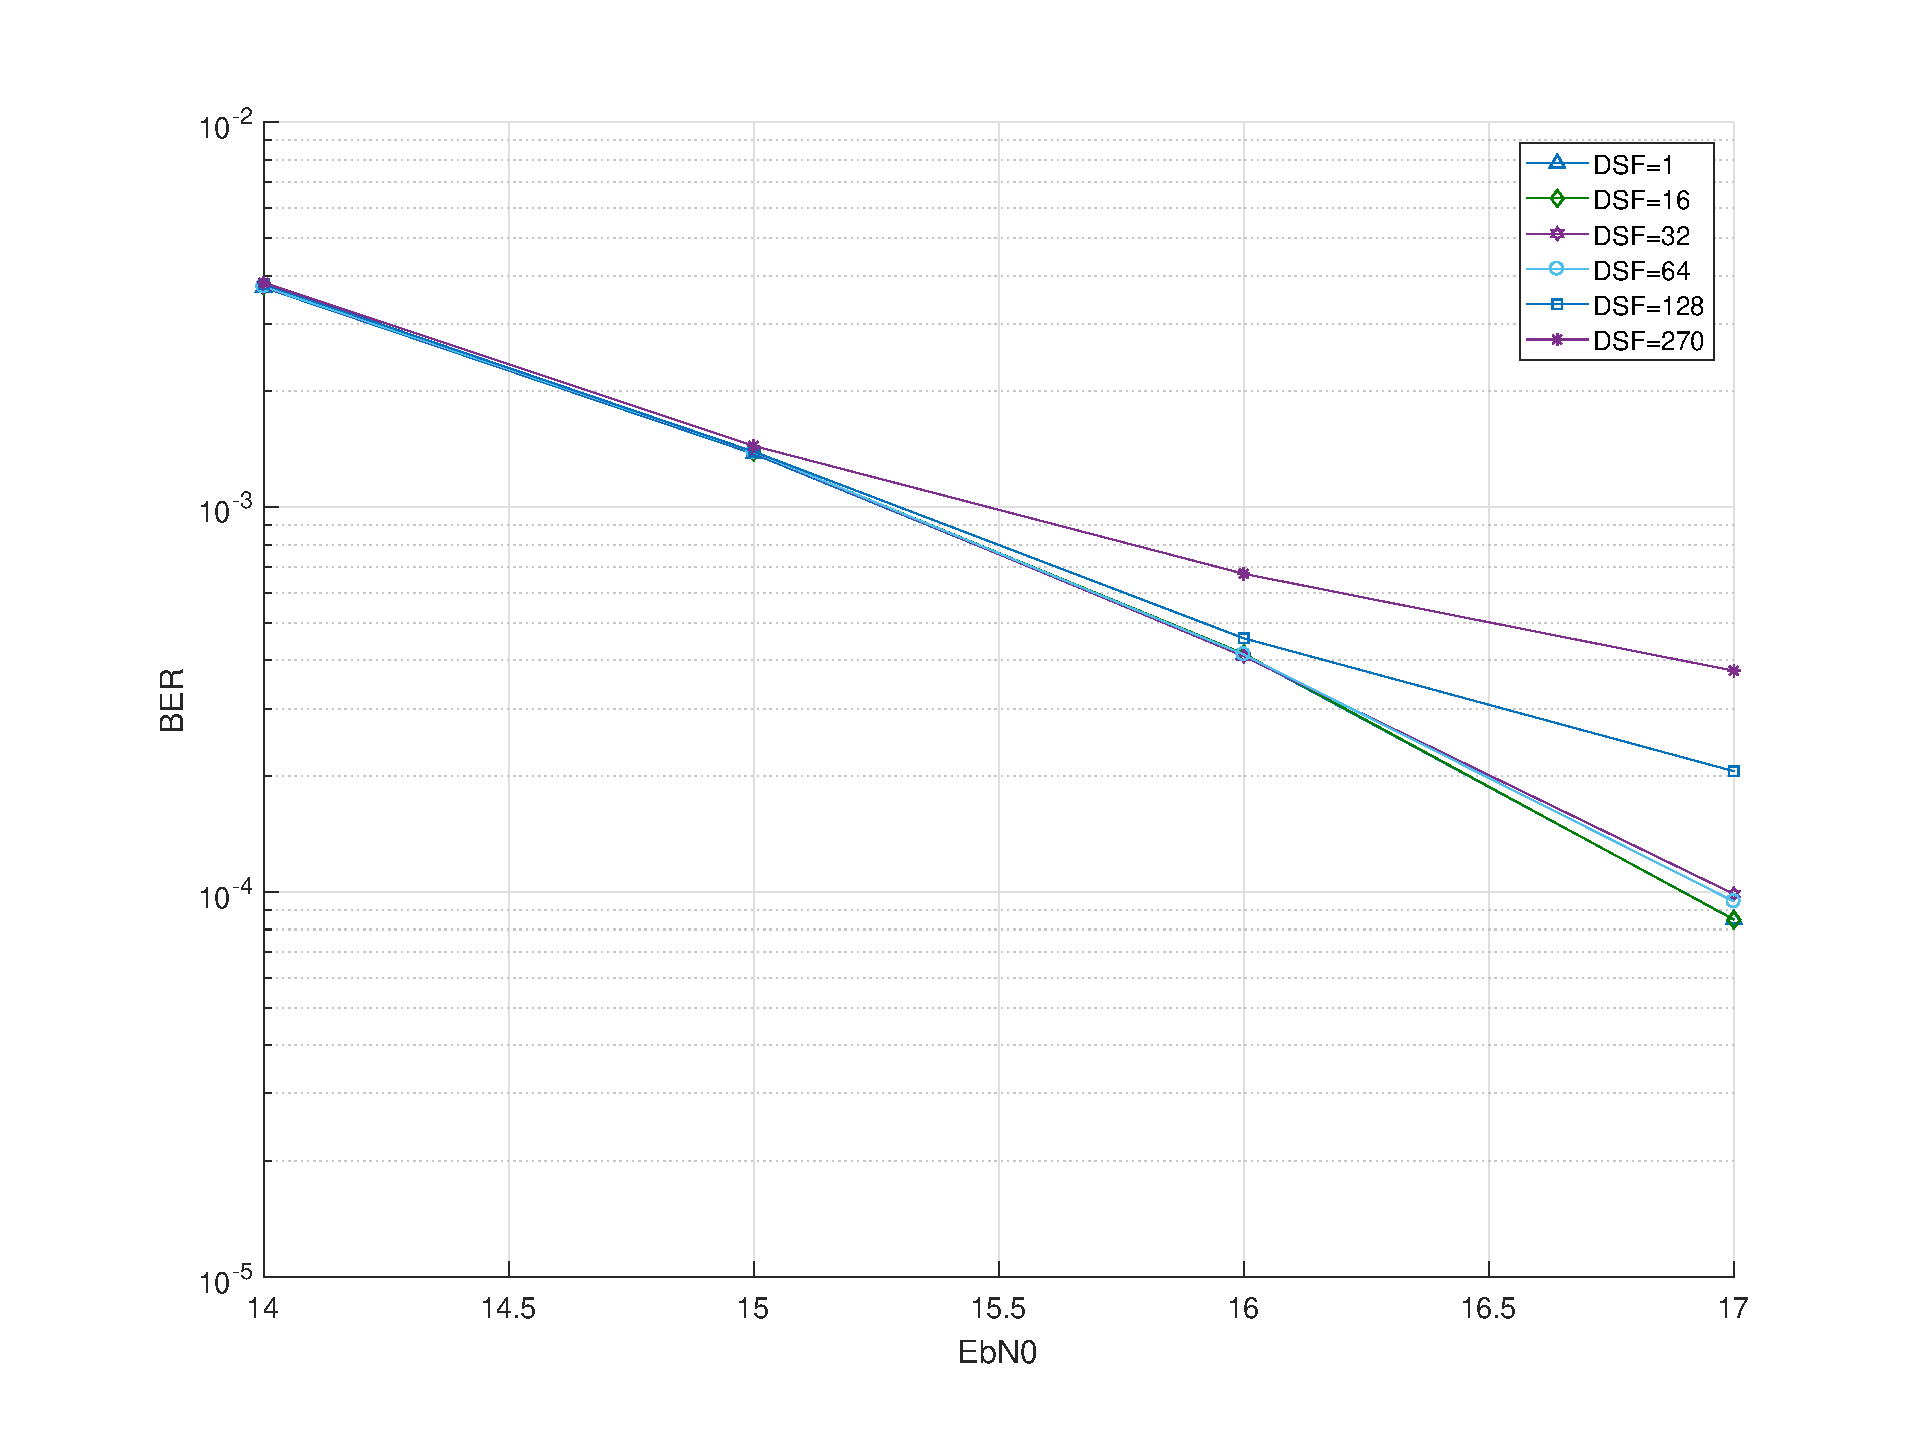
\includegraphics[width=0.85\textwidth]{figures/fig_red_kalman/xpic_xpd_25_qam_64_bis.eps}
	\caption{BER for 2-state Kalman with different DSF. $64$-QAM, $XPD=25$ dB, pilot interval=56.}
	\label{fig13}      
\end{figure}

\begin{figure}
	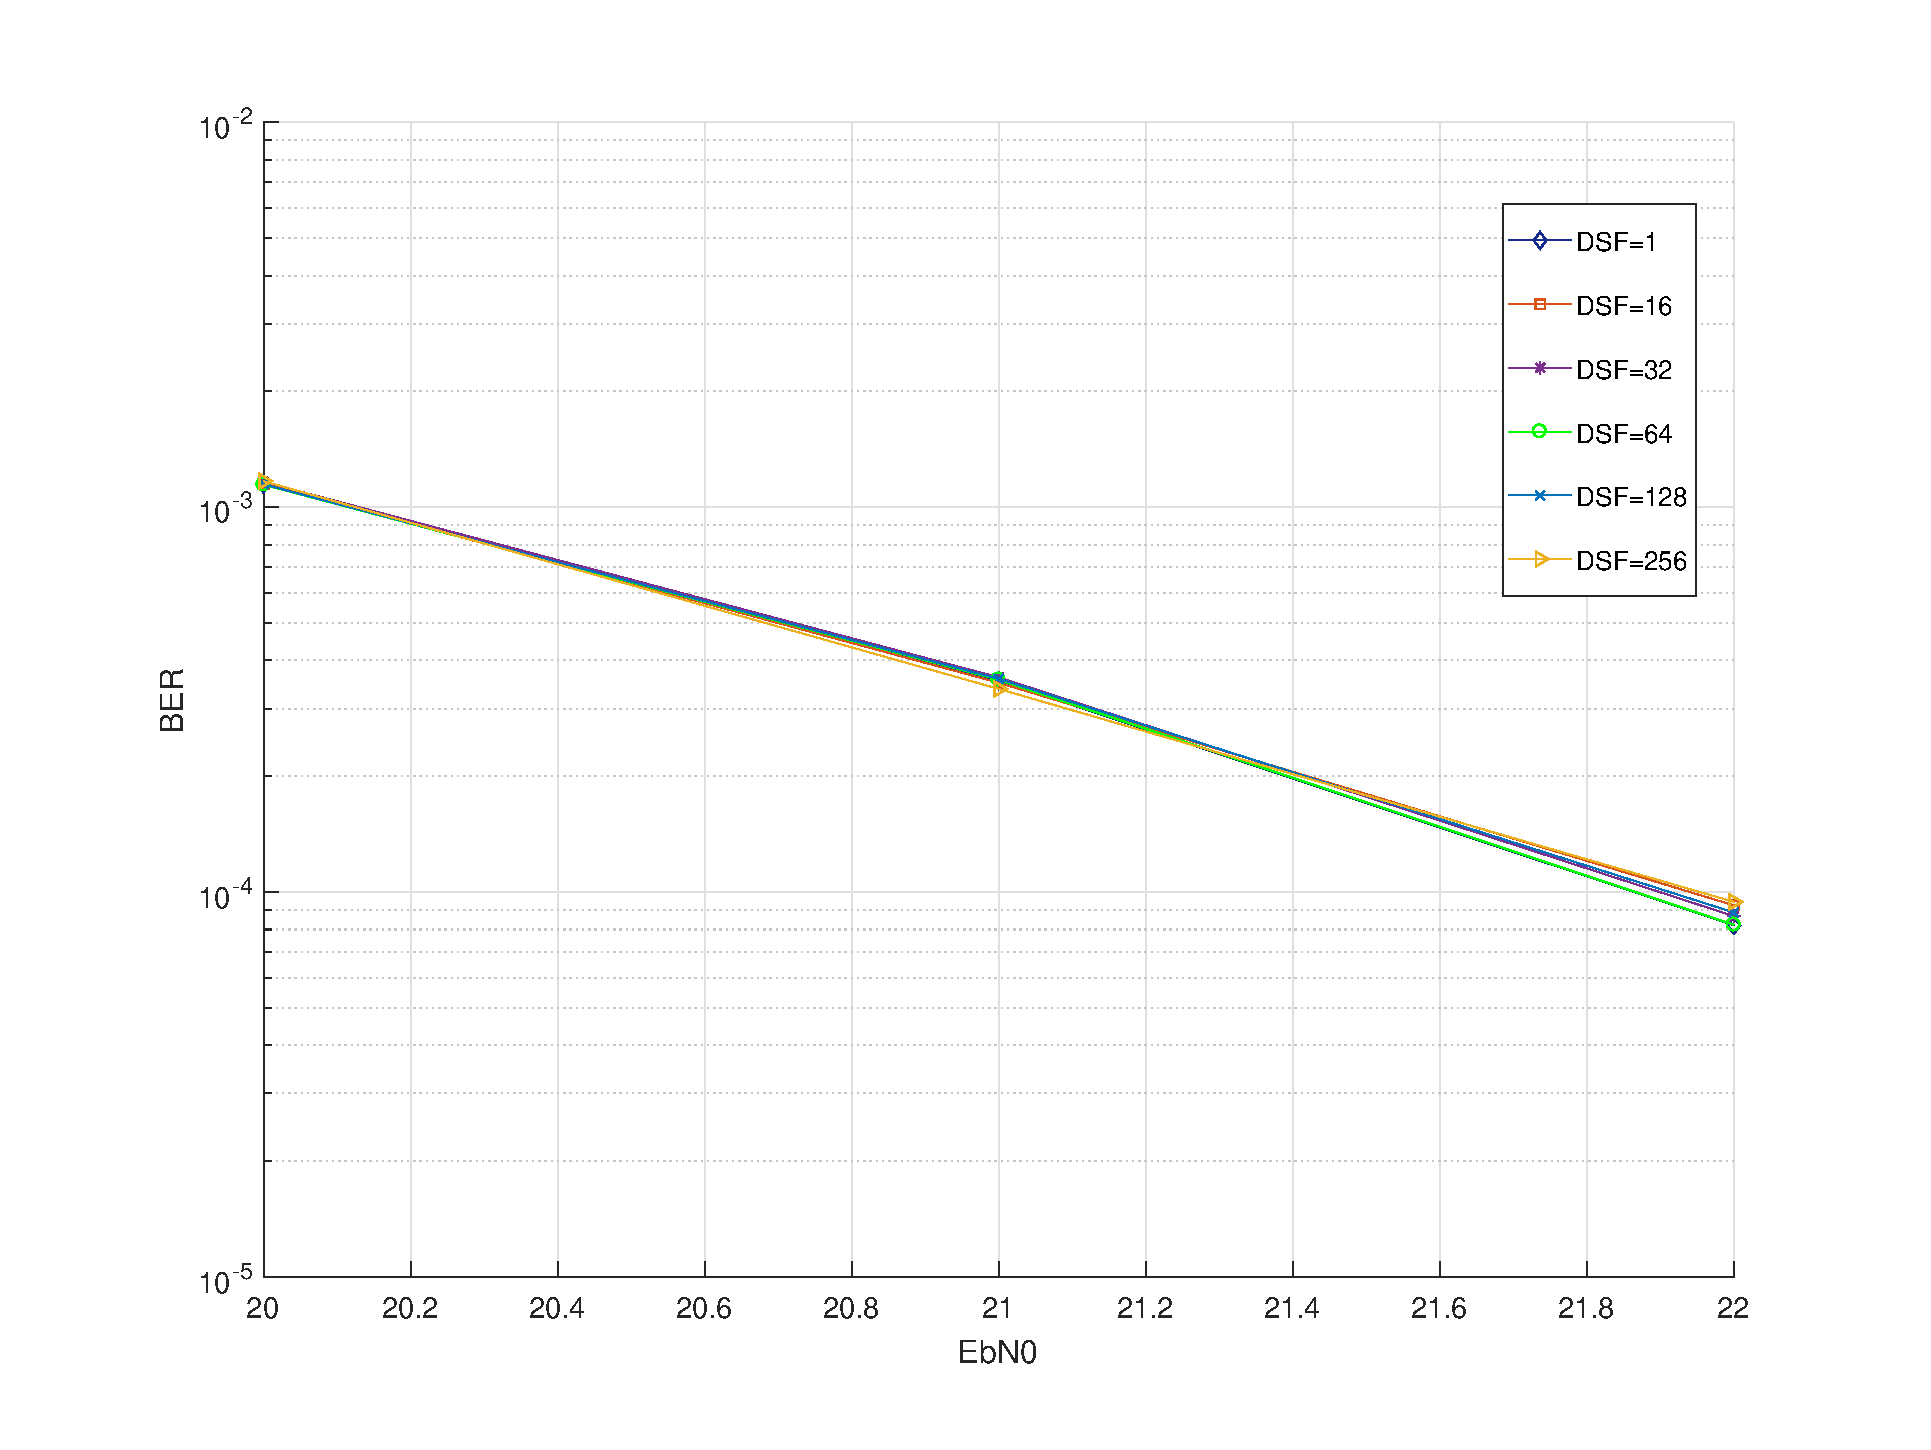
\includegraphics[width=0.85\textwidth]{figures/fig_red_kalman/xpic_xpd_15_qam_256_bis.eps}
	\caption{BER for 2-state Kalman with different DSF. $256$-QAM, $XPD=15$ dB, pilot interval=56.}
	\label{fig14}      
\end{figure}

\begin{figure}
	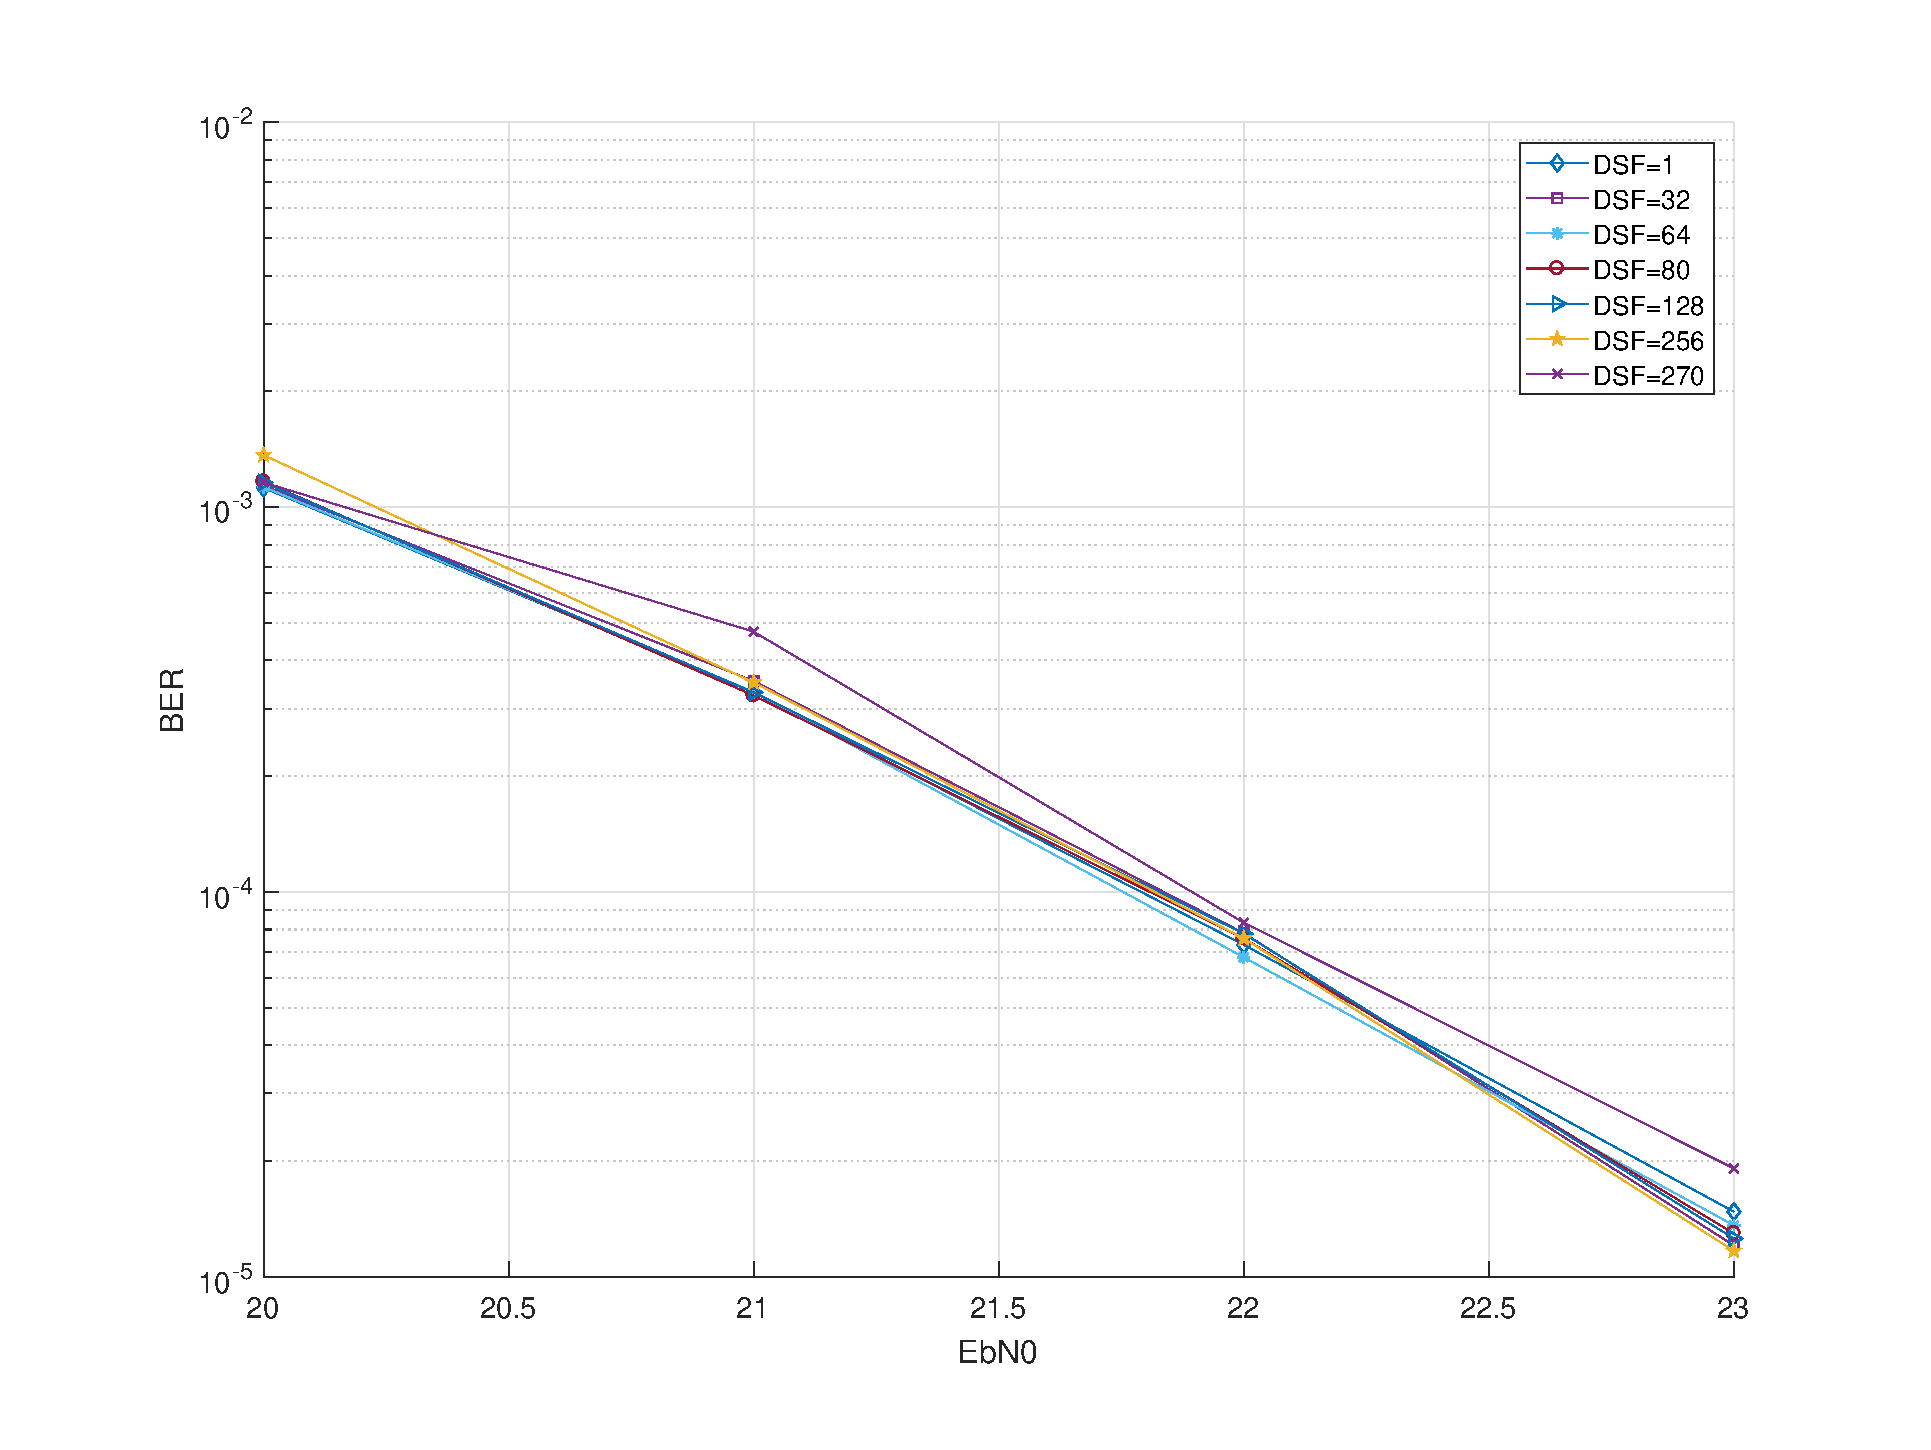
\includegraphics[width=0.85\textwidth]{figures/fig_red_kalman/xpic_xpd_25_qam_256_bis.eps}
	\caption{BER for 2-state Kalman with different DSF. $256$-QAM, $XPD=25$ dB, pilot interval=56.}
	\label{fig15}      
\end{figure}
\section{Conclusion}
\label{Concl}
In this work we have considered a cross-polarized communications system based on two independent transceiver chains, in order to have the maximum flexibility from an installation and maintenance point of view, to connect different single carrier transceivers to dual-polarized antennas.
A new solution has been proposed to recover the phase of the two horizontal and vertical signals on the cross-polar radio links by exploiting a reduced complexity one-state Kalman filter. Moreover, an alternative error detection computation and the covariance matrix loop downsampling have been proposed.
Simulations results prove the effectiveness of the proposed reduced complexity Kalman based solutions, whose main benefit is to directly adapt its parameters according to new channel noise and interference conditions showing better performance of the \textcolor{black}{commonly} used second-order PLL scheme. 
Indeed, the commonly used PLL solution needs to optimize and re-set its parameters each time. On this purpose, we have also developed a relation between the EKF filter and PLL scheme envisioning a solution where a Kalman based algorithm optimizes off-line the PLL parameters for the cross-polar interference canceler. Since the proposed complexity reduction schemes may be applied not only\textcolor{black}{to the EKF, but also to the other types of Kalman algorithms, such as the unscented filter \cite{Wan2000}, as future works we are going to address other Kalman architectures as well as hardware experimental results.} 
